% Options for packages loaded elsewhere
\PassOptionsToPackage{unicode}{hyperref}
\PassOptionsToPackage{hyphens}{url}
%
\documentclass[
]{article}
\usepackage{amsmath,amssymb}
\usepackage{iftex}
\ifPDFTeX
  \usepackage[T1]{fontenc}
  \usepackage[utf8]{inputenc}
  \usepackage{textcomp} % provide euro and other symbols
\else % if luatex or xetex
  \usepackage{unicode-math} % this also loads fontspec
  \defaultfontfeatures{Scale=MatchLowercase}
  \defaultfontfeatures[\rmfamily]{Ligatures=TeX,Scale=1}
\fi
\usepackage{lmodern}
\ifPDFTeX\else
  % xetex/luatex font selection
\fi
% Use upquote if available, for straight quotes in verbatim environments
\IfFileExists{upquote.sty}{\usepackage{upquote}}{}
\IfFileExists{microtype.sty}{% use microtype if available
  \usepackage[]{microtype}
  \UseMicrotypeSet[protrusion]{basicmath} % disable protrusion for tt fonts
}{}
\makeatletter
\@ifundefined{KOMAClassName}{% if non-KOMA class
  \IfFileExists{parskip.sty}{%
    \usepackage{parskip}
  }{% else
    \setlength{\parindent}{0pt}
    \setlength{\parskip}{6pt plus 2pt minus 1pt}}
}{% if KOMA class
  \KOMAoptions{parskip=half}}
\makeatother
\usepackage{xcolor}
\usepackage[margin=1in]{geometry}
\usepackage{color}
\usepackage{fancyvrb}
\newcommand{\VerbBar}{|}
\newcommand{\VERB}{\Verb[commandchars=\\\{\}]}
\DefineVerbatimEnvironment{Highlighting}{Verbatim}{commandchars=\\\{\}}
% Add ',fontsize=\small' for more characters per line
\usepackage{framed}
\definecolor{shadecolor}{RGB}{248,248,248}
\newenvironment{Shaded}{\begin{snugshade}}{\end{snugshade}}
\newcommand{\AlertTok}[1]{\textcolor[rgb]{0.94,0.16,0.16}{#1}}
\newcommand{\AnnotationTok}[1]{\textcolor[rgb]{0.56,0.35,0.01}{\textbf{\textit{#1}}}}
\newcommand{\AttributeTok}[1]{\textcolor[rgb]{0.13,0.29,0.53}{#1}}
\newcommand{\BaseNTok}[1]{\textcolor[rgb]{0.00,0.00,0.81}{#1}}
\newcommand{\BuiltInTok}[1]{#1}
\newcommand{\CharTok}[1]{\textcolor[rgb]{0.31,0.60,0.02}{#1}}
\newcommand{\CommentTok}[1]{\textcolor[rgb]{0.56,0.35,0.01}{\textit{#1}}}
\newcommand{\CommentVarTok}[1]{\textcolor[rgb]{0.56,0.35,0.01}{\textbf{\textit{#1}}}}
\newcommand{\ConstantTok}[1]{\textcolor[rgb]{0.56,0.35,0.01}{#1}}
\newcommand{\ControlFlowTok}[1]{\textcolor[rgb]{0.13,0.29,0.53}{\textbf{#1}}}
\newcommand{\DataTypeTok}[1]{\textcolor[rgb]{0.13,0.29,0.53}{#1}}
\newcommand{\DecValTok}[1]{\textcolor[rgb]{0.00,0.00,0.81}{#1}}
\newcommand{\DocumentationTok}[1]{\textcolor[rgb]{0.56,0.35,0.01}{\textbf{\textit{#1}}}}
\newcommand{\ErrorTok}[1]{\textcolor[rgb]{0.64,0.00,0.00}{\textbf{#1}}}
\newcommand{\ExtensionTok}[1]{#1}
\newcommand{\FloatTok}[1]{\textcolor[rgb]{0.00,0.00,0.81}{#1}}
\newcommand{\FunctionTok}[1]{\textcolor[rgb]{0.13,0.29,0.53}{\textbf{#1}}}
\newcommand{\ImportTok}[1]{#1}
\newcommand{\InformationTok}[1]{\textcolor[rgb]{0.56,0.35,0.01}{\textbf{\textit{#1}}}}
\newcommand{\KeywordTok}[1]{\textcolor[rgb]{0.13,0.29,0.53}{\textbf{#1}}}
\newcommand{\NormalTok}[1]{#1}
\newcommand{\OperatorTok}[1]{\textcolor[rgb]{0.81,0.36,0.00}{\textbf{#1}}}
\newcommand{\OtherTok}[1]{\textcolor[rgb]{0.56,0.35,0.01}{#1}}
\newcommand{\PreprocessorTok}[1]{\textcolor[rgb]{0.56,0.35,0.01}{\textit{#1}}}
\newcommand{\RegionMarkerTok}[1]{#1}
\newcommand{\SpecialCharTok}[1]{\textcolor[rgb]{0.81,0.36,0.00}{\textbf{#1}}}
\newcommand{\SpecialStringTok}[1]{\textcolor[rgb]{0.31,0.60,0.02}{#1}}
\newcommand{\StringTok}[1]{\textcolor[rgb]{0.31,0.60,0.02}{#1}}
\newcommand{\VariableTok}[1]{\textcolor[rgb]{0.00,0.00,0.00}{#1}}
\newcommand{\VerbatimStringTok}[1]{\textcolor[rgb]{0.31,0.60,0.02}{#1}}
\newcommand{\WarningTok}[1]{\textcolor[rgb]{0.56,0.35,0.01}{\textbf{\textit{#1}}}}
\usepackage{longtable,booktabs,array}
\usepackage{calc} % for calculating minipage widths
% Correct order of tables after \paragraph or \subparagraph
\usepackage{etoolbox}
\makeatletter
\patchcmd\longtable{\par}{\if@noskipsec\mbox{}\fi\par}{}{}
\makeatother
% Allow footnotes in longtable head/foot
\IfFileExists{footnotehyper.sty}{\usepackage{footnotehyper}}{\usepackage{footnote}}
\makesavenoteenv{longtable}
\usepackage{graphicx}
\makeatletter
\def\maxwidth{\ifdim\Gin@nat@width>\linewidth\linewidth\else\Gin@nat@width\fi}
\def\maxheight{\ifdim\Gin@nat@height>\textheight\textheight\else\Gin@nat@height\fi}
\makeatother
% Scale images if necessary, so that they will not overflow the page
% margins by default, and it is still possible to overwrite the defaults
% using explicit options in \includegraphics[width, height, ...]{}
\setkeys{Gin}{width=\maxwidth,height=\maxheight,keepaspectratio}
% Set default figure placement to htbp
\makeatletter
\def\fps@figure{htbp}
\makeatother
\setlength{\emergencystretch}{3em} % prevent overfull lines
\providecommand{\tightlist}{%
  \setlength{\itemsep}{0pt}\setlength{\parskip}{0pt}}
\setcounter{secnumdepth}{5}
\ifLuaTeX
  \usepackage{selnolig}  % disable illegal ligatures
\fi
\IfFileExists{bookmark.sty}{\usepackage{bookmark}}{\usepackage{hyperref}}
\IfFileExists{xurl.sty}{\usepackage{xurl}}{} % add URL line breaks if available
\urlstyle{same}
\hypersetup{
  pdftitle={Bitcoin candlestick predictions using lagged features and machine learning algorithm in R},
  pdfauthor={Sandoche Adittane},
  hidelinks,
  pdfcreator={LaTeX via pandoc}}

\title{Bitcoin candlestick predictions using lagged features and machine
learning algorithm in R}
\usepackage{etoolbox}
\makeatletter
\providecommand{\subtitle}[1]{% add subtitle to \maketitle
  \apptocmd{\@title}{\par {\large #1 \par}}{}{}
}
\makeatother
\subtitle{Training various machine learning algorithms to predict the
next candlestick of the bitcoin price using various lagged features}
\author{Sandoche Adittane}
\date{2025-04-17}

\begin{document}
\maketitle
\begin{abstract}
This report explores how to get the best accuracy on predicting the next
candlestick of the bitcoin chart using the previous ones. It compares
different algorithms: Generalized Linear Model, Decision Tree, Random
Forest, KNN and Gradient boosting and different number of lagged
features. This project is part of the `Data Science: Capstone' module of
HarvardX PH125.9x from the edx platform.
\end{abstract}

\newpage
\tableofcontents
\listoffigures
\listoftables
\newpage

\hypertarget{overview}{%
\section{Overview}\label{overview}}

In this study we will try to predict the direction of the next
candlestick of the bitcoin chart. Before starting, it's important to
understand what are Bitcoin, candlesticks and what is the goal of this
study.

\hypertarget{introduction-to-bitcoin}{%
\subsection{Introduction to Bitcoin}\label{introduction-to-bitcoin}}

This last years Bitcoin (BTC) has been gaining attention not only by
retail investors but also by institutional investor. In 2025 we've seen
the emergence of spot Bitcoin exchange-traded funds (ETF) from
institutions such as BlackRock, VanEck, Grayscale. With a market
capitalization of about 1.68 billion in dollars at the time of writing,
Bitcoin started as a peer-to-peer currency, a free alernative to
centralized currencies controlled by central banks. It is now used more
as an investment, a store of value and even considered as a strategic
reserve assets by some countries.

TODO: Add examples with sources.

Bitcoin ows is decentralization and to it's data structure, the
blockchain, a chain of block that contains transaction, and to its
consensus, the proof of work. Without going too much into details, it
makes a Bitcoin a currency that does not rely on a centralized server.
Proof of work is a cryptographic competition where the Bitcoin servers
called nodes compete to decide which one is the next block to be added
to the blockchain. They go through a process called mining where nodes
have to use their computing power to find a number called nonce. This
computing power is called the hashrate. The node who succeed at
``mining'' successfully gets rewarded for that.

TODO: reference to my article

The fact that Bitcoin is defined by its codebase is quite facinating,
also having all its ledger visible and publically available gives a lot
of data available to analyze. Moreover unlike stocks BTC can be traded
any time, there is no opening or closing hours, the bitcoin market never
stops and it is very easy for anyone to buy and sell bitcoin. Those are
two reasons worth studying bitcoin's candlestick charts instead of other
asset.

\hypertarget{what-are-candlesticks}{%
\subsection{What are candlesticks?}\label{what-are-candlesticks}}

Let's talk about the candlestick. The price of assets such as bitcoin is
described by a serie of candle stick defined by, an opening price, a
close price a high and a low also called OHLC. A candlestick can be
``up'' / ``bullish'' if closing price is higher than opening price, or
``down'' / ``bearish'' otherwise. You can see this visually with the
following figure. ``\,''

\url{https://i0.wp.com/techqualitypedia.com/wp-content/uploads/2024/09/candlestick-components.jpg?w=1491\&ssl=1}
Source: \url{https://techqualitypedia.com/candlestick-patterns-bullish/}

The candle stick chart is defined as a time serie of candles, each
candle is defined at a defined time and have a time duration. We will
explain more in detail in the exploratory analysis.

\hypertarget{candlesticks-pattern}{%
\subsection{Candlesticks pattern}\label{candlesticks-pattern}}

TODO Talk about chartists and common patterns

\hypertarget{goal-of-the-study}{%
\subsection{Goal of the study}\label{goal-of-the-study}}

The goal of the study is to find a model able to predict the direction
of a candlestick using N previous candles. This number N will be also
part of the research. We will have to not only find N but also find what
are the best features to achieve the best accuracy.

\hypertarget{applications}{%
\subsection{Applications}\label{applications}}

Why is the direction of a candlestick matter? Because being able to
predict the direction of the next candle could enable trader to buy and
sell on spot market when the predicted candle is green. Also perpetual
futures trader can go both way, they can long when the prediction says
``up'' and ``short'' when the predictions says ``down''.

TODO: Give some resource to learn about spot vs future.

\hypertarget{exploratory-data-analysis}{%
\section{Exploratory data analysis}\label{exploratory-data-analysis}}

In this section we will see what are the are the different dataset
available, see what features are available to train the different
models, prepare the data, verify it, and choose different machine
learning algorithms we will use and compare.

\hypertarget{data-sets}{%
\subsection{Data sets}\label{data-sets}}

In order to conduct this study we used as a the main data set the
historic rates for the trading pair BTC-USD using Coinbase API. TODO:
add reference
\url{https://docs.cdp.coinbase.com/exchange/reference/exchangerestapi_getproductcandles}

We used the following global variables for the full project:

\begin{Shaded}
\begin{Highlighting}[]
\NormalTok{trading\_pair }\OtherTok{\textless{}{-}} \StringTok{"BTC{-}USD"}
\NormalTok{start\_date }\OtherTok{\textless{}{-}} \StringTok{"2024{-}01{-}01"}
\NormalTok{end\_date }\OtherTok{\textless{}{-}} \StringTok{"2025{-}03{-}29"}
\NormalTok{candlestick\_period }\OtherTok{\textless{}{-}} \DecValTok{3600}
\FunctionTok{set.seed}\NormalTok{(}\DecValTok{1}\NormalTok{)}
\end{Highlighting}
\end{Shaded}

The timeframe is the entire year 2024 and the start of the year 2025
until the day we started the study. Note that since January 2024,
Bitcoin ETF has officially been approved. The period
\texttt{candlestick\_period\ \textless{}-\ 3600} is the time of a
candle, the candle closes 1h after it starts. Which means we have 24
candles per day.

I choose this settings to have a dataset of around 10000 candles but
also since Bitcoin ETF has been approved the market may have taken a
different dynamic than the previous years.

Let's see how the dataset looks like.

\begin{longtable}[]{@{}lrrrrr@{}}
\caption{Overview of the BTC-USD candlestick dataset}\tabularnewline
\toprule\noalign{}
time & low & high & open & close & volume \\
\midrule\noalign{}
\endfirsthead
\toprule\noalign{}
time & low & high & open & close & volume \\
\midrule\noalign{}
\endhead
\bottomrule\noalign{}
\endlastfoot
2024-01-01 00:00:00 & 42261.58 & 42543.64 & 42288.58 & 42452.66 &
379.1973 \\
2024-01-01 01:00:00 & 42415.00 & 42749.99 & 42453.83 & 42594.68 &
396.2019 \\
2024-01-01 02:00:00 & 42488.03 & 42625.68 & 42594.58 & 42571.32 &
227.1412 \\
2024-01-01 03:00:00 & 42235.00 & 42581.26 & 42571.32 & 42325.11 &
306.0057 \\
2024-01-01 04:00:00 & 42200.00 & 42393.48 & 42325.10 & 42389.77 &
296.2336 \\
2024-01-01 05:00:00 & 42175.65 & 42396.09 & 42389.78 & 42231.47 &
188.1280 \\
\end{longtable}

We have 10,873 entries in our candle stick dataset. As described in the
overview it contains the OCLH data, timestamp and the volume of each
candles.

Bitcoin is used by 3 types of users:

\begin{itemize}
\item
  Traders --- they are interested by the price and make profit
\item
  Users --- using the currency to do payments or to transfer money
  around the world
\item
  Miners --- they mine bitcoin to sell it, their interest is that the
  price of bitcoin is higher than the cost of mining bitcoin
\end{itemize}

Keeping this in mind, I tried to find other dataset that could represent
each of the type of users that could eventually help in our predictions
and I picked the following:

\begin{itemize}
\item
  Fear and greed index --- represents the overall mood of the market
  (traders)
\item
  Hash-rate --- defines the overall mining power (miners)
\item
  Average block size --- the higher it is the more transactions are
  happening (users)
\item
  Number of transactions --- defines the activity of the network (users)
\item
  Number of unspent transaction outputs (UTXO) --- defines how many
  addresses contains bitcoin, and reflects the network activity (users)
\end{itemize}

\url{https://www.blockchain.com/explorer/charts/total-bitcoins}
\url{https://alternative.me/crypto/fear-and-greed-index/}

\begin{Shaded}
\begin{Highlighting}[]
\NormalTok{fear\_and\_greed\_index }\OtherTok{\textless{}{-}} \FunctionTok{read\_csv}\NormalTok{(}\FunctionTok{paste0}\NormalTok{(}\StringTok{"data/"}\NormalTok{, trading\_pair,}
    \StringTok{"\_fear\_and\_greed\_index\_"}\NormalTok{, start\_date, }\StringTok{"\_"}\NormalTok{, end\_date, }\StringTok{".csv"}\NormalTok{))}
\end{Highlighting}
\end{Shaded}

\begin{verbatim}
## Rows: 453 Columns: 3
## -- Column specification --------------------------------------------------------
## Delimiter: ","
## chr  (1): value_classification
## dbl  (1): value
## dttm (1): timestamp
## 
## i Use `spec()` to retrieve the full column specification for this data.
## i Specify the column types or set `show_col_types = FALSE` to quiet this message.
\end{verbatim}

\begin{Shaded}
\begin{Highlighting}[]
\NormalTok{fear\_and\_greed\_index }\OtherTok{\textless{}{-}}\NormalTok{ fear\_and\_greed\_index }\SpecialCharTok{\%\textgreater{}\%}
    \FunctionTok{mutate}\NormalTok{(}\AttributeTok{value =} \FunctionTok{as.numeric}\NormalTok{(value))}
\NormalTok{knitr}\SpecialCharTok{::}\FunctionTok{kable}\NormalTok{(}\FunctionTok{head}\NormalTok{(fear\_and\_greed\_index), }\AttributeTok{format =} \StringTok{"simple"}\NormalTok{, }\AttributeTok{caption =} \StringTok{"Overview of the BTC fear and greed index dataset"}\NormalTok{)}
\end{Highlighting}
\end{Shaded}

\begin{longtable}[]{@{}rll@{}}
\caption{Overview of the BTC fear and greed index
dataset}\tabularnewline
\toprule\noalign{}
value & value\_classification & timestamp \\
\midrule\noalign{}
\endfirsthead
\toprule\noalign{}
value & value\_classification & timestamp \\
\midrule\noalign{}
\endhead
\bottomrule\noalign{}
\endlastfoot
26 & Fear & 2025-03-29 \\
44 & Fear & 2025-03-28 \\
40 & Fear & 2025-03-27 \\
47 & Neutral & 2025-03-26 \\
46 & Fear & 2025-03-25 \\
45 & Fear & 2025-03-24 \\
\end{longtable}

This dataset is a time serie of the daily fear and greed index, it is a
value between 0 and 100, 0 being the most fearful and 100 being the most
greedy. The data set contains 453 entries.

\begin{Shaded}
\begin{Highlighting}[]
\NormalTok{hash\_rate }\OtherTok{\textless{}{-}}\NormalTok{ jsonlite}\SpecialCharTok{::}\FunctionTok{fromJSON}\NormalTok{(}\StringTok{"data/hash{-}rate.json"}\NormalTok{)}\SpecialCharTok{$}\StringTok{\textasciigrave{}}\AttributeTok{hash{-}rate}\StringTok{\textasciigrave{}} \SpecialCharTok{\%\textgreater{}\%}
    \FunctionTok{rename}\NormalTok{(}\AttributeTok{timestamp =}\NormalTok{ x, }\AttributeTok{hash\_rate =}\NormalTok{ y) }\SpecialCharTok{\%\textgreater{}\%}
    \FunctionTok{mutate}\NormalTok{(}\AttributeTok{timestamp =} \FunctionTok{as.POSIXct}\NormalTok{(timestamp}\SpecialCharTok{/}\DecValTok{1000}\NormalTok{, }\AttributeTok{origin =} \StringTok{"1970{-}01{-}01"}\NormalTok{,}
        \AttributeTok{tz =} \StringTok{"UTC"}\NormalTok{)) }\SpecialCharTok{\%\textgreater{}\%}
    \FunctionTok{filter}\NormalTok{(timestamp }\SpecialCharTok{\textgreater{}=} \FunctionTok{as.POSIXct}\NormalTok{(start\_date, }\AttributeTok{origin =} \StringTok{"1970{-}01{-}01"}\NormalTok{,}
        \AttributeTok{tz =} \StringTok{"UTC"}\NormalTok{) }\SpecialCharTok{\&}\NormalTok{ timestamp }\SpecialCharTok{\textless{}=} \FunctionTok{as.POSIXct}\NormalTok{(end\_date, }\AttributeTok{origin =} \StringTok{"1970{-}01{-}01"}\NormalTok{,}
        \AttributeTok{tz =} \StringTok{"UTC"}\NormalTok{))}
\NormalTok{knitr}\SpecialCharTok{::}\FunctionTok{kable}\NormalTok{(}\FunctionTok{head}\NormalTok{(hash\_rate), }\AttributeTok{format =} \StringTok{"simple"}\NormalTok{, }\AttributeTok{caption =} \StringTok{"Overview of the BTC hash rate dataset"}\NormalTok{)}
\end{Highlighting}
\end{Shaded}

\begin{longtable}[]{@{}lr@{}}
\caption{Overview of the BTC hash rate dataset}\tabularnewline
\toprule\noalign{}
timestamp & hash\_rate \\
\midrule\noalign{}
\endfirsthead
\toprule\noalign{}
timestamp & hash\_rate \\
\midrule\noalign{}
\endhead
\bottomrule\noalign{}
\endlastfoot
2024-01-01 & 501122294 \\
2024-01-02 & 509303882 \\
2024-01-03 & 505213088 \\
2024-01-04 & 520042217 \\
2024-01-05 & 545098332 \\
2024-01-06 & 538450791 \\
\end{longtable}

This dataset is a time serie of the daily hash rate, it is a value in
TH/s. The data set contains 454 entries.

\begin{Shaded}
\begin{Highlighting}[]
\NormalTok{average\_block\_size }\OtherTok{\textless{}{-}}\NormalTok{ jsonlite}\SpecialCharTok{::}\FunctionTok{fromJSON}\NormalTok{(}\StringTok{"data/avg{-}block{-}size.json"}\NormalTok{)}\SpecialCharTok{$}\StringTok{\textasciigrave{}}\AttributeTok{avg{-}block{-}size}\StringTok{\textasciigrave{}} \SpecialCharTok{\%\textgreater{}\%}
    \FunctionTok{rename}\NormalTok{(}\AttributeTok{timestamp =}\NormalTok{ x, }\AttributeTok{avg\_block\_size =}\NormalTok{ y) }\SpecialCharTok{\%\textgreater{}\%}
    \FunctionTok{mutate}\NormalTok{(}\AttributeTok{timestamp =} \FunctionTok{as.POSIXct}\NormalTok{(timestamp}\SpecialCharTok{/}\DecValTok{1000}\NormalTok{, }\AttributeTok{origin =} \StringTok{"1970{-}01{-}01"}\NormalTok{,}
        \AttributeTok{tz =} \StringTok{"UTC"}\NormalTok{)) }\SpecialCharTok{\%\textgreater{}\%}
    \FunctionTok{filter}\NormalTok{(timestamp }\SpecialCharTok{\textgreater{}=} \FunctionTok{as.POSIXct}\NormalTok{(start\_date, }\AttributeTok{origin =} \StringTok{"1970{-}01{-}01"}\NormalTok{,}
        \AttributeTok{tz =} \StringTok{"UTC"}\NormalTok{) }\SpecialCharTok{\&}\NormalTok{ timestamp }\SpecialCharTok{\textless{}=} \FunctionTok{as.POSIXct}\NormalTok{(end\_date, }\AttributeTok{origin =} \StringTok{"1970{-}01{-}01"}\NormalTok{,}
        \AttributeTok{tz =} \StringTok{"UTC"}\NormalTok{))}
\NormalTok{knitr}\SpecialCharTok{::}\FunctionTok{kable}\NormalTok{(}\FunctionTok{head}\NormalTok{(average\_block\_size), }\AttributeTok{format =} \StringTok{"simple"}\NormalTok{, }\AttributeTok{caption =} \StringTok{"Overview of the BTC average block size dataset"}\NormalTok{)}
\end{Highlighting}
\end{Shaded}

\begin{longtable}[]{@{}lr@{}}
\caption{Overview of the BTC average block size dataset}\tabularnewline
\toprule\noalign{}
timestamp & avg\_block\_size \\
\midrule\noalign{}
\endfirsthead
\toprule\noalign{}
timestamp & avg\_block\_size \\
\midrule\noalign{}
\endhead
\bottomrule\noalign{}
\endlastfoot
2024-01-01 & 1.653640 \\
2024-01-02 & 1.718455 \\
2024-01-03 & 1.771466 \\
2024-01-04 & 1.782402 \\
2024-01-05 & 1.774551 \\
2024-01-06 & 1.847959 \\
\end{longtable}

This dataset is a time serie of the daily average block size, it is a
value in bytes. The data set contains 454 entries.

\begin{Shaded}
\begin{Highlighting}[]
\NormalTok{n\_transactions }\OtherTok{\textless{}{-}}\NormalTok{ jsonlite}\SpecialCharTok{::}\FunctionTok{fromJSON}\NormalTok{(}\StringTok{"data/n{-}transactions.json"}\NormalTok{)}\SpecialCharTok{$}\StringTok{\textasciigrave{}}\AttributeTok{n{-}transactions}\StringTok{\textasciigrave{}} \SpecialCharTok{\%\textgreater{}\%}
    \FunctionTok{rename}\NormalTok{(}\AttributeTok{timestamp =}\NormalTok{ x, }\AttributeTok{n\_transactions =}\NormalTok{ y) }\SpecialCharTok{\%\textgreater{}\%}
    \FunctionTok{mutate}\NormalTok{(}\AttributeTok{timestamp =} \FunctionTok{as.POSIXct}\NormalTok{(timestamp}\SpecialCharTok{/}\DecValTok{1000}\NormalTok{, }\AttributeTok{origin =} \StringTok{"1970{-}01{-}01"}\NormalTok{,}
        \AttributeTok{tz =} \StringTok{"UTC"}\NormalTok{)) }\SpecialCharTok{\%\textgreater{}\%}
    \FunctionTok{filter}\NormalTok{(timestamp }\SpecialCharTok{\textgreater{}=} \FunctionTok{as.POSIXct}\NormalTok{(start\_date, }\AttributeTok{origin =} \StringTok{"1970{-}01{-}01"}\NormalTok{,}
        \AttributeTok{tz =} \StringTok{"UTC"}\NormalTok{) }\SpecialCharTok{\&}\NormalTok{ timestamp }\SpecialCharTok{\textless{}=} \FunctionTok{as.POSIXct}\NormalTok{(end\_date, }\AttributeTok{origin =} \StringTok{"1970{-}01{-}01"}\NormalTok{,}
        \AttributeTok{tz =} \StringTok{"UTC"}\NormalTok{))}
\NormalTok{knitr}\SpecialCharTok{::}\FunctionTok{kable}\NormalTok{(}\FunctionTok{head}\NormalTok{(n\_transactions), }\AttributeTok{format =} \StringTok{"simple"}\NormalTok{, }\AttributeTok{caption =} \StringTok{"Overview of the BTC number of transactions dataset"}\NormalTok{)}
\end{Highlighting}
\end{Shaded}

\begin{longtable}[]{@{}lr@{}}
\caption{Overview of the BTC number of transactions
dataset}\tabularnewline
\toprule\noalign{}
timestamp & n\_transactions \\
\midrule\noalign{}
\endfirsthead
\toprule\noalign{}
timestamp & n\_transactions \\
\midrule\noalign{}
\endhead
\bottomrule\noalign{}
\endlastfoot
2024-01-01 & 657752 \\
2024-01-02 & 367319 \\
2024-01-03 & 502749 \\
2024-01-04 & 482557 \\
2024-01-05 & 420884 \\
2024-01-06 & 382140 \\
\end{longtable}

This dataset is a time serie of the daily number of transactions, it is
a value in transactions. The data set contains 454 entries.

\begin{Shaded}
\begin{Highlighting}[]
\NormalTok{utxo\_count }\OtherTok{\textless{}{-}}\NormalTok{ jsonlite}\SpecialCharTok{::}\FunctionTok{fromJSON}\NormalTok{(}\StringTok{"data/utxo{-}count.json"}\NormalTok{)}\SpecialCharTok{$}\StringTok{\textasciigrave{}}\AttributeTok{utxo{-}count}\StringTok{\textasciigrave{}} \SpecialCharTok{\%\textgreater{}\%}
    \FunctionTok{rename}\NormalTok{(}\AttributeTok{timestamp =}\NormalTok{ x, }\AttributeTok{utxo\_count =}\NormalTok{ y) }\SpecialCharTok{\%\textgreater{}\%}
    \FunctionTok{mutate}\NormalTok{(}\AttributeTok{timestamp =} \FunctionTok{as.POSIXct}\NormalTok{(timestamp}\SpecialCharTok{/}\DecValTok{1000}\NormalTok{, }\AttributeTok{origin =} \StringTok{"1970{-}01{-}01"}\NormalTok{,}
        \AttributeTok{tz =} \StringTok{"UTC"}\NormalTok{), }\AttributeTok{timestamp =} \FunctionTok{as.Date}\NormalTok{(timestamp)) }\SpecialCharTok{\%\textgreater{}\%}
    \FunctionTok{filter}\NormalTok{(timestamp }\SpecialCharTok{\textgreater{}=} \FunctionTok{as.Date}\NormalTok{(start\_date) }\SpecialCharTok{\&}\NormalTok{ timestamp }\SpecialCharTok{\textless{}=} \FunctionTok{as.Date}\NormalTok{(end\_date)) }\SpecialCharTok{\%\textgreater{}\%}
    \FunctionTok{group\_by}\NormalTok{(timestamp) }\SpecialCharTok{\%\textgreater{}\%}
    \FunctionTok{summarise}\NormalTok{(}\AttributeTok{utxo\_count =} \FunctionTok{mean}\NormalTok{(utxo\_count))  }\CommentTok{\# Take average for each date}
\NormalTok{knitr}\SpecialCharTok{::}\FunctionTok{kable}\NormalTok{(}\FunctionTok{head}\NormalTok{(utxo\_count), }\AttributeTok{format =} \StringTok{"simple"}\NormalTok{, }\AttributeTok{caption =} \StringTok{"Overview of the BTC UTXO count dataset"}\NormalTok{)}
\end{Highlighting}
\end{Shaded}

\begin{longtable}[]{@{}lr@{}}
\caption{Overview of the BTC UTXO count dataset}\tabularnewline
\toprule\noalign{}
timestamp & utxo\_count \\
\midrule\noalign{}
\endfirsthead
\toprule\noalign{}
timestamp & utxo\_count \\
\midrule\noalign{}
\endhead
\bottomrule\noalign{}
\endlastfoot
2024-01-01 & 135878807 \\
2024-01-02 & 136204295 \\
2024-01-03 & 136536575 \\
2024-01-04 & 136871780 \\
2024-01-05 & 137209298 \\
2024-01-06 & 137552822 \\
\end{longtable}

This dataset is a time serie of the daily number of UTXO, it is the
count of UTXO in the network. The data set contains 454 entries. We had
to group by timestamp since some dates had more than 1 value.

As we can see \texttt{fear\_and\_greed\_index} seems to miss one data
point. We will see fix that in the next sections.

We have different dataset that we will use for the predictions but we
are still missing one important data used by traders, technical analysis
indicator.

Based on a previous research and blog post I wrote, I decided to include
a few indicators that are very common in trading:

\begin{itemize}
\item
  Moving average convergence divergence (MACD)
\item
  Rate of change (ROC)
\item
  Bolinger Bands (BB)
\item
  Relative Strenght Index (RSI)
\end{itemize}

TODO: add
\url{https://medium.com/learning-lab/become-a-better-crypto-trader-with-technical-and-chart-analysis-1496b2fc6b85}

Before preparing the dataset let's see what would be the features we can
extract from the OHLC candlestick data.

\hypertarget{features}{%
\subsection{Features}\label{features}}

Our candlesticks dataset from coinbase gives us values that are based on
the price of bitcoin, but used itself for a machine learning algorithm
it will be hard to use those raw absolute values since the price always
fluctuate, so we have to think about what defines the candlesticks we
have seen above?

If we isolate a candle we can see the following features:

\begin{itemize}
\item
  Size of the body
\item
  Size of the upper shadow / wicks
\item
  Size of the lower shadow / wicks
\item
  Direction of the candle (up or down)
\item
  Closing price
\end{itemize}

We are now ready to prepare the dataset for the study.

\hypertarget{preparation}{%
\subsection{Preparation}\label{preparation}}

\begin{Shaded}
\begin{Highlighting}[]
\NormalTok{enhance\_dataset }\OtherTok{\textless{}{-}} \ControlFlowTok{function}\NormalTok{(candles\_data, fear\_and\_greed\_index\_data, hash\_rate\_data, average\_block\_size\_data, n\_transactions\_data, utxo\_count\_data) \{}
\NormalTok{  candles\_enhanced }\OtherTok{\textless{}{-}}\NormalTok{ candles\_data }\SpecialCharTok{\%\textgreater{}\%}
    \FunctionTok{mutate}\NormalTok{(}\AttributeTok{date\_only =} \FunctionTok{as.Date}\NormalTok{(time)) }\SpecialCharTok{\%\textgreater{}\%}
    \FunctionTok{left\_join}\NormalTok{(fear\_and\_greed\_index\_data, }\AttributeTok{by =} \FunctionTok{c}\NormalTok{(}\StringTok{"date\_only"} \OtherTok{=} \StringTok{"timestamp"}\NormalTok{)) }\SpecialCharTok{\%\textgreater{}\%}
    \FunctionTok{left\_join}\NormalTok{(hash\_rate\_data, }\AttributeTok{by =} \FunctionTok{c}\NormalTok{(}\StringTok{"date\_only"} \OtherTok{=} \StringTok{"timestamp"}\NormalTok{)) }\SpecialCharTok{\%\textgreater{}\%}
    \FunctionTok{left\_join}\NormalTok{(average\_block\_size\_data, }\AttributeTok{by =} \FunctionTok{c}\NormalTok{(}\StringTok{"date\_only"} \OtherTok{=} \StringTok{"timestamp"}\NormalTok{)) }\SpecialCharTok{\%\textgreater{}\%}
    \FunctionTok{left\_join}\NormalTok{(n\_transactions\_data, }\AttributeTok{by =} \FunctionTok{c}\NormalTok{(}\StringTok{"date\_only"} \OtherTok{=} \StringTok{"timestamp"}\NormalTok{)) }\SpecialCharTok{\%\textgreater{}\%}
    \FunctionTok{left\_join}\NormalTok{(utxo\_count\_data, }\AttributeTok{by =} \FunctionTok{c}\NormalTok{(}\StringTok{"date\_only"} \OtherTok{=} \StringTok{"timestamp"}\NormalTok{)) }\SpecialCharTok{\%\textgreater{}\%}
    \FunctionTok{mutate}\NormalTok{(}
      \AttributeTok{body\_size =} \FunctionTok{abs}\NormalTok{(close }\SpecialCharTok{{-}}\NormalTok{ open),}
      \AttributeTok{upper\_shadow\_size =}\NormalTok{ high }\SpecialCharTok{{-}} \FunctionTok{pmax}\NormalTok{(close, open),}
      \AttributeTok{lower\_shadow\_size =} \FunctionTok{pmin}\NormalTok{(close, open) }\SpecialCharTok{{-}}\NormalTok{ low,}
      \AttributeTok{direction =} \FunctionTok{ifelse}\NormalTok{(close }\SpecialCharTok{\textgreater{}}\NormalTok{ open, }\StringTok{"up"}\NormalTok{, }\StringTok{"down"}\NormalTok{),}
\NormalTok{    ) }\SpecialCharTok{\%\textgreater{}\%}
    \FunctionTok{tq\_mutate}\NormalTok{(}
      \AttributeTok{select =}\NormalTok{ close,}
      \AttributeTok{mutate\_fun =}\NormalTok{ ROC,}
      \AttributeTok{n =} \DecValTok{14}\NormalTok{,}
      \AttributeTok{col\_rename =} \StringTok{"roc"}
\NormalTok{    ) }\SpecialCharTok{\%\textgreater{}\%}
    \FunctionTok{tq\_mutate}\NormalTok{( }\CommentTok{\# https://www.keenbase{-}trading.com/find{-}best{-}macd{-}settings/\#t{-}1719588154943}
      \AttributeTok{select =}\NormalTok{ close,}
      \AttributeTok{mutate\_fun =}\NormalTok{ MACD,}
      \AttributeTok{nFast =} \DecValTok{12}\NormalTok{,}
      \AttributeTok{nSlow =} \DecValTok{26}\NormalTok{,}
      \AttributeTok{nSig =} \DecValTok{9}\NormalTok{,}
      \AttributeTok{col\_rename =} \FunctionTok{c}\NormalTok{(}\StringTok{"macd"}\NormalTok{, }\StringTok{"signal"}\NormalTok{)}
\NormalTok{    ) }\SpecialCharTok{\%\textgreater{}\%}
    \FunctionTok{tq\_mutate}\NormalTok{(}
      \AttributeTok{select =}\NormalTok{ close,}
      \AttributeTok{mutate\_fun =}\NormalTok{ RSI,}
      \AttributeTok{n =} \DecValTok{14}\NormalTok{,}
      \AttributeTok{col\_rename =} \StringTok{"rsi"}
\NormalTok{    ) }\SpecialCharTok{\%\textgreater{}\%}
    \FunctionTok{tq\_mutate}\NormalTok{(}
      \AttributeTok{select =}\NormalTok{ close,}
      \AttributeTok{mutate\_fun =}\NormalTok{ BBands,}
      \AttributeTok{n =} \DecValTok{20}\NormalTok{,}
      \AttributeTok{sd =} \DecValTok{2}\NormalTok{,}
      \AttributeTok{col\_rename =} \StringTok{"bband"}
\NormalTok{    )}

\NormalTok{  candles\_enhanced}
\NormalTok{\}}

\NormalTok{candles\_enhanced }\OtherTok{\textless{}{-}} \FunctionTok{enhance\_dataset}\NormalTok{(candles, fear\_and\_greed\_index, hash\_rate, average\_block\_size, n\_transactions, utxo\_count)}
\end{Highlighting}
\end{Shaded}

\begin{verbatim}
## Warning in coerce_to_tibble(ret, date_col_name, time_zone, col_rename): Could not rename columns. The function name will be used. 
##   Is the length of `col_rename` the same as the number of columns returned from the `mutate_fun`?
\end{verbatim}

\begin{Shaded}
\begin{Highlighting}[]
\NormalTok{knitr}\SpecialCharTok{::}\FunctionTok{kable}\NormalTok{(}\FunctionTok{head}\NormalTok{(candles\_enhanced), }\AttributeTok{format =} \StringTok{"simple"}\NormalTok{, }\AttributeTok{caption =} \StringTok{"Overview of the candlestick dataset enhanced"}\NormalTok{)}
\end{Highlighting}
\end{Shaded}

\begin{longtable}[]{@{}lrrrrrlrlrrrrrrrlrrrrrrrr@{}}
\caption{Overview of the candlestick dataset enhanced}\tabularnewline
\toprule\noalign{}
time & low & high & open & close & volume & date\_only & value &
value\_classification & hash\_rate & avg\_block\_size & n\_transactions
& utxo\_count & body\_size & upper\_shadow\_size & lower\_shadow\_size &
direction & roc & macd & signal & rsi & dn & mavg & up & pctB \\
\midrule\noalign{}
\endfirsthead
\toprule\noalign{}
time & low & high & open & close & volume & date\_only & value &
value\_classification & hash\_rate & avg\_block\_size & n\_transactions
& utxo\_count & body\_size & upper\_shadow\_size & lower\_shadow\_size &
direction & roc & macd & signal & rsi & dn & mavg & up & pctB \\
\midrule\noalign{}
\endhead
\bottomrule\noalign{}
\endlastfoot
2024-01-01 00:00:00 & 42261.58 & 42543.64 & 42288.58 & 42452.66 &
379.1973 & 2024-01-01 & 65 & Greed & 501122294 & 1.65364 & 657752 &
135878807 & 164.08 & 90.98 & 27.00 & up & NA & NA & NA & NA & NA & NA &
NA & NA \\
2024-01-01 01:00:00 & 42415.00 & 42749.99 & 42453.83 & 42594.68 &
396.2019 & 2024-01-01 & 65 & Greed & 501122294 & 1.65364 & 657752 &
135878807 & 140.85 & 155.31 & 38.83 & up & NA & NA & NA & NA & NA & NA &
NA & NA \\
2024-01-01 02:00:00 & 42488.03 & 42625.68 & 42594.58 & 42571.32 &
227.1412 & 2024-01-01 & 65 & Greed & 501122294 & 1.65364 & 657752 &
135878807 & 23.26 & 31.10 & 83.29 & down & NA & NA & NA & NA & NA & NA &
NA & NA \\
2024-01-01 03:00:00 & 42235.00 & 42581.26 & 42571.32 & 42325.11 &
306.0057 & 2024-01-01 & 65 & Greed & 501122294 & 1.65364 & 657752 &
135878807 & 246.21 & 9.94 & 90.11 & down & NA & NA & NA & NA & NA & NA &
NA & NA \\
2024-01-01 04:00:00 & 42200.00 & 42393.48 & 42325.10 & 42389.77 &
296.2336 & 2024-01-01 & 65 & Greed & 501122294 & 1.65364 & 657752 &
135878807 & 64.67 & 3.71 & 125.10 & up & NA & NA & NA & NA & NA & NA &
NA & NA \\
2024-01-01 05:00:00 & 42175.65 & 42396.09 & 42389.78 & 42231.47 &
188.1280 & 2024-01-01 & 65 & Greed & 501122294 & 1.65364 & 657752 &
135878807 & 158.31 & 6.31 & 55.82 & down & NA & NA & NA & NA & NA & NA &
NA & NA \\
\end{longtable}

We have now a table with all the features discussed above. Before adding
the lagged features let's explore our set.

First let's see if we have NAs.

\begin{Shaded}
\begin{Highlighting}[]
\NormalTok{na\_indexes }\OtherTok{\textless{}{-}} \FunctionTok{which}\NormalTok{(}\FunctionTok{apply}\NormalTok{(candles\_enhanced, }\DecValTok{1}\NormalTok{, }\ControlFlowTok{function}\NormalTok{(x) }\FunctionTok{any}\NormalTok{(}\FunctionTok{is.na}\NormalTok{(x))))}
\NormalTok{knitr}\SpecialCharTok{::}\FunctionTok{kable}\NormalTok{(candles\_enhanced[na\_indexes, ], }\AttributeTok{format =} \StringTok{"simple"}\NormalTok{,}
    \AttributeTok{caption =} \StringTok{"NAs of the dataset"}\NormalTok{)}
\end{Highlighting}
\end{Shaded}

\begin{longtable}[]{@{}lrrrrrlrlrrrrrrrlrrrrrrrr@{}}
\caption{NAs of the dataset}\tabularnewline
\toprule\noalign{}
time & low & high & open & close & volume & date\_only & value &
value\_classification & hash\_rate & avg\_block\_size & n\_transactions
& utxo\_count & body\_size & upper\_shadow\_size & lower\_shadow\_size &
direction & roc & macd & signal & rsi & dn & mavg & up & pctB \\
\midrule\noalign{}
\endfirsthead
\toprule\noalign{}
time & low & high & open & close & volume & date\_only & value &
value\_classification & hash\_rate & avg\_block\_size & n\_transactions
& utxo\_count & body\_size & upper\_shadow\_size & lower\_shadow\_size &
direction & roc & macd & signal & rsi & dn & mavg & up & pctB \\
\midrule\noalign{}
\endhead
\bottomrule\noalign{}
\endlastfoot
2024-01-01 00:00:00 & 42261.58 & 42543.64 & 42288.58 & 42452.66 &
379.197253 & 2024-01-01 & 65 & Greed & 501122294 & 1.653640 & 657752 &
135878807 & 164.08 & 90.98 & 27.00 & up & NA & NA & NA & NA & NA & NA &
NA & NA \\
2024-01-01 01:00:00 & 42415.00 & 42749.99 & 42453.83 & 42594.68 &
396.201924 & 2024-01-01 & 65 & Greed & 501122294 & 1.653640 & 657752 &
135878807 & 140.85 & 155.31 & 38.83 & up & NA & NA & NA & NA & NA & NA &
NA & NA \\
2024-01-01 02:00:00 & 42488.03 & 42625.68 & 42594.58 & 42571.32 &
227.141166 & 2024-01-01 & 65 & Greed & 501122294 & 1.653640 & 657752 &
135878807 & 23.26 & 31.10 & 83.29 & down & NA & NA & NA & NA & NA & NA &
NA & NA \\
2024-01-01 03:00:00 & 42235.00 & 42581.26 & 42571.32 & 42325.11 &
306.005694 & 2024-01-01 & 65 & Greed & 501122294 & 1.653640 & 657752 &
135878807 & 246.21 & 9.94 & 90.11 & down & NA & NA & NA & NA & NA & NA &
NA & NA \\
2024-01-01 04:00:00 & 42200.00 & 42393.48 & 42325.10 & 42389.77 &
296.233644 & 2024-01-01 & 65 & Greed & 501122294 & 1.653640 & 657752 &
135878807 & 64.67 & 3.71 & 125.10 & up & NA & NA & NA & NA & NA & NA &
NA & NA \\
2024-01-01 05:00:00 & 42175.65 & 42396.09 & 42389.78 & 42231.47 &
188.128033 & 2024-01-01 & 65 & Greed & 501122294 & 1.653640 & 657752 &
135878807 & 158.31 & 6.31 & 55.82 & down & NA & NA & NA & NA & NA & NA &
NA & NA \\
2024-01-01 06:00:00 & 42199.63 & 42463.83 & 42231.47 & 42400.90 &
327.010976 & 2024-01-01 & 65 & Greed & 501122294 & 1.653640 & 657752 &
135878807 & 169.43 & 62.93 & 31.84 & up & NA & NA & NA & NA & NA & NA &
NA & NA \\
2024-01-01 07:00:00 & 42396.80 & 42534.49 & 42400.90 & 42496.49 &
407.835097 & 2024-01-01 & 65 & Greed & 501122294 & 1.653640 & 657752 &
135878807 & 95.59 & 38.00 & 4.10 & up & NA & NA & NA & NA & NA & NA & NA
& NA \\
2024-01-01 08:00:00 & 42451.00 & 42560.26 & 42496.58 & 42552.70 &
134.066714 & 2024-01-01 & 65 & Greed & 501122294 & 1.653640 & 657752 &
135878807 & 56.12 & 7.56 & 45.58 & up & NA & NA & NA & NA & NA & NA & NA
& NA \\
2024-01-01 09:00:00 & 42533.77 & 42692.84 & 42552.70 & 42650.97 &
128.157349 & 2024-01-01 & 65 & Greed & 501122294 & 1.653640 & 657752 &
135878807 & 98.27 & 41.87 & 18.93 & up & NA & NA & NA & NA & NA & NA &
NA & NA \\
2024-01-01 10:00:00 & 42625.75 & 42750.00 & 42650.97 & 42688.50 &
118.457396 & 2024-01-01 & 65 & Greed & 501122294 & 1.653640 & 657752 &
135878807 & 37.53 & 61.50 & 25.22 & up & NA & NA & NA & NA & NA & NA &
NA & NA \\
2024-01-01 11:00:00 & 42598.94 & 42767.60 & 42686.73 & 42690.00 &
135.177672 & 2024-01-01 & 65 & Greed & 501122294 & 1.653640 & 657752 &
135878807 & 3.27 & 77.60 & 87.79 & up & NA & NA & NA & NA & NA & NA & NA
& NA \\
2024-01-01 12:00:00 & 42610.77 & 42778.74 & 42690.00 & 42647.83 &
143.378020 & 2024-01-01 & 65 & Greed & 501122294 & 1.653640 & 657752 &
135878807 & 42.17 & 88.74 & 37.06 & down & NA & NA & NA & NA & NA & NA &
NA & NA \\
2024-01-01 13:00:00 & 42608.98 & 42750.00 & 42647.85 & 42715.88 &
101.798625 & 2024-01-01 & 65 & Greed & 501122294 & 1.653640 & 657752 &
135878807 & 68.03 & 34.12 & 38.87 & up & NA & NA & NA & NA & NA & NA &
NA & NA \\
2024-01-01 14:00:00 & 42581.54 & 42723.28 & 42717.53 & 42635.19 &
254.331002 & 2024-01-01 & 65 & Greed & 501122294 & 1.653640 & 657752 &
135878807 & 82.34 & 5.75 & 53.65 & down & 0.0042904 & NA & NA & 57.10792
& NA & NA & NA & NA \\
2024-01-01 15:00:00 & 42601.88 & 42868.74 & 42633.57 & 42797.33 &
323.614895 & 2024-01-01 & 65 & Greed & 501122294 & 1.653640 & 657752 &
135878807 & 163.76 & 71.41 & 31.69 & up & 0.0047464 & NA & NA & 62.24262
& NA & NA & NA & NA \\
2024-01-01 16:00:00 & 42680.01 & 42880.97 & 42799.37 & 42742.35 &
330.024110 & 2024-01-01 & 65 & Greed & 501122294 & 1.653640 & 657752 &
135878807 & 57.02 & 81.60 & 62.34 & down & 0.0040094 & NA & NA &
59.63561 & NA & NA & NA & NA \\
2024-01-01 17:00:00 & 42720.76 & 42846.42 & 42738.88 & 42833.66 &
254.872245 & 2024-01-01 & 65 & Greed & 501122294 & 1.653640 & 657752 &
135878807 & 94.78 & 12.76 & 18.12 & up & 0.0119437 & NA & NA & 62.44867
& NA & NA & NA & NA \\
2024-01-01 18:00:00 & 42835.63 & 43228.37 & 42835.63 & 43120.92 &
625.461696 & 2024-01-01 & 65 & Greed & 501122294 & 1.653640 & 657752 &
135878807 & 285.29 & 107.45 & 0.00 & up & 0.0171012 & NA & NA & 69.62147
& NA & NA & NA & NA \\
2024-01-01 19:00:00 & 43106.97 & 43567.46 & 43123.82 & 43547.61 &
506.451809 & 2024-01-01 & 65 & Greed & 501122294 & 1.653640 & 657752 &
135878807 & 423.79 & 19.85 & 16.85 & up & 0.0306891 & NA & NA & 76.73127
& 42090.27 & 42654.27 & 43218.26 & 1.2919817 \\
2024-01-01 20:00:00 & 43537.04 & 43849.90 & 43537.04 & 43701.58 &
559.329005 & 2024-01-01 & 65 & Greed & 501122294 & 1.653640 & 657752 &
135878807 & 164.54 & 148.32 & 0.00 & up & 0.0302147 & NA & NA & 78.67112
& 41999.96 & 42716.71 & 43433.46 & 1.1870350 \\
2024-01-01 21:00:00 & 43467.97 & 43800.00 & 43703.06 & 43632.21 &
313.991915 & 2024-01-01 & 65 & Greed & 501122294 & 1.653640 & 657752 &
135878807 & 70.85 & 96.94 & 164.24 & down & 0.0263742 & NA & NA &
75.61261 & 41951.51 & 42768.59 & 43585.67 & 1.0284809 \\
2024-01-01 22:00:00 & 43389.00 & 43677.06 & 43631.79 & 43546.06 &
247.539449 & 2024-01-01 & 65 & Greed & 501122294 & 1.653640 & 657752 &
135878807 & 85.73 & 45.27 & 157.06 & down & 0.0230759 & NA & NA &
71.87544 & 41939.13 & 42817.33 & 43695.52 & 0.9149046 \\
2024-01-01 23:00:00 & 43545.99 & 44240.80 & 43545.99 & 44220.78 &
1273.322823 & 2024-01-01 & 65 & Greed & 501122294 & 1.653640 & 657752 &
135878807 & 674.79 & 20.02 & 0.00 & up & 0.0361448 & NA & NA & 80.15023
& 41872.51 & 42912.11 & 43951.71 & 1.1294098 \\
2024-01-02 00:00:00 & 44195.13 & 45250.00 & 44220.78 & 45093.17 &
3023.793096 & 2024-01-02 & 71 & Greed & 509303882 & 1.718455 & 367319 &
136204295 & 872.39 & 156.83 & 25.65 & up & 0.0548012 & NA & NA &
85.91894 & 41667.24 & 43047.28 & 44427.32 & 1.2412405 \\
2024-01-02 01:00:00 & 44714.89 & 45417.45 & 45093.14 & 44894.58 &
1983.082789 & 2024-01-02 & 71 & Greed & 509303882 & 1.718455 & 367319 &
136204295 & 198.56 & 324.31 & 179.69 & down & 0.0503524 & 1.8270330 & NA
& 80.20475 & 41636.74 & 43180.44 & 44724.13 & 1.0552081 \\
2024-01-02 02:00:00 & 44891.40 & 45500.00 & 44891.41 & 45485.31 &
1913.577949 & 2024-01-02 & 71 & Greed & 509303882 & 1.718455 & 367319 &
136204295 & 593.90 & 14.69 & 0.01 & up & 0.0644130 & 1.9971797 & NA &
83.68143 & 41537.77 & 43334.66 & 45131.55 & 1.0984378 \\
2024-01-02 03:00:00 & 45178.34 & 45601.00 & 45485.32 & 45473.97 &
1512.833935 & 2024-01-02 & 71 & Greed & 509303882 & 1.718455 & 367319 &
136204295 & 11.35 & 115.68 & 295.63 & down & 0.0625693 & 2.1034776 & NA
& 83.37869 & 41504.90 & 43483.53 & 45462.16 & 1.0029836 \\
2024-01-02 04:00:00 & 45204.47 & 45544.10 & 45476.27 & 45218.83 &
681.159462 & 2024-01-02 & 71 & Greed & 509303882 & 1.718455 & 367319 &
136204295 & 257.44 & 67.83 & 14.36 & down & 0.0588336 & 2.1152334 & NA &
76.65897 & 41549.74 & 43616.84 & 45683.93 & 0.8874993 \\
2024-01-02 05:00:00 & 45131.00 & 45370.54 & 45218.84 & 45216.32 &
484.732085 & 2024-01-02 & 71 & Greed & 509303882 & 1.718455 & 367319 &
136204295 & 2.52 & 151.70 & 85.32 & down & 0.0549824 & 2.0989517 & NA &
76.59357 & 41616.22 & 43745.10 & 45873.99 & 0.8455368 \\
2024-01-02 06:00:00 & 45166.39 & 45361.61 & 45214.41 & 45208.54 &
495.637602 & 2024-01-02 & 71 & Greed & 509303882 & 1.718455 & 367319 &
136204295 & 5.87 & 147.20 & 42.15 & down & 0.0560958 & 2.0601496 & NA &
76.37608 & 41709.23 & 43871.11 & 46032.98 & 0.8093231 \\
2024-01-02 07:00:00 & 45209.48 & 45707.69 & 45209.48 & 45504.64 &
976.921273 & 2024-01-02 & 71 & Greed & 509303882 & 1.718455 & 367319 &
136204295 & 295.16 & 203.05 & 0.00 & up & 0.0604901 & 2.0585375 & NA &
78.83895 & 41809.76 & 44011.84 & 46213.92 & 0.8389528 \\
2024-01-02 08:00:00 & 45382.34 & 45899.96 & 45504.40 & 45808.07 &
759.882169 & 2024-01-02 & 71 & Greed & 509303882 & 1.718455 & 367319 &
136204295 & 303.67 & 91.89 & 122.06 & up & 0.0604520 & 2.0869707 & NA &
81.02236 & 41928.76 & 44169.85 & 46410.94 & 0.8654968 \\
2024-10-26 00:00:00 & 66413.18 & 66754.02 & 66564.51 & 66635.55 &
359.487900 & 2024-10-26 & NA & NA & 735533947 & 1.719950 & 597744 &
186546028 & 71.04 & 118.47 & 151.33 & up & -0.0175694 & -0.4043104 &
-0.2103219 & 38.06098 & 66252.00 & 67399.29 & 68546.58 & 0.1671540 \\
2024-10-26 01:00:00 & 66430.80 & 66711.88 & 66637.60 & 66597.10 &
226.587448 & 2024-10-26 & NA & NA & 735533947 & 1.719950 & 597744 &
186546028 & 40.50 & 74.28 & 166.30 & down & -0.0218030 & -0.4256175 &
-0.2533810 & 37.54739 & 66154.79 & 67343.84 & 68532.90 & 0.1859938 \\
2024-10-26 02:00:00 & 66331.95 & 66930.14 & 66594.88 & 66728.09 &
162.061446 & 2024-10-26 & NA & NA & 735533947 & 1.719950 & 597744 &
186546028 & 133.21 & 202.05 & 262.93 & up & -0.0192072 & -0.4219183 &
-0.2870885 & 40.49336 & 66088.25 & 67300.64 & 68513.04 & 0.2638747 \\
2024-10-26 03:00:00 & 66580.85 & 66890.00 & 66730.12 & 66816.54 &
122.871792 & 2024-10-26 & NA & NA & 735533947 & 1.719950 & 597744 &
186546028 & 86.42 & 73.46 & 149.27 & up & -0.0216914 & -0.4036971 &
-0.3104102 & 42.46687 & 66040.00 & 67266.33 & 68492.66 & 0.3166112 \\
2024-10-26 04:00:00 & 66687.79 & 66903.91 & 66814.44 & 66855.95 &
148.712344 & 2024-10-26 & NA & NA & 735533947 & 1.719950 & 597744 &
186546028 & 41.51 & 47.96 & 126.65 & up & -0.0209919 & -0.3801337 &
-0.3243549 & 43.36809 & 66000.50 & 67228.68 & 68456.86 & 0.3482580 \\
2024-10-26 05:00:00 & 66851.79 & 67156.74 & 66855.94 & 67049.34 &
163.124225 & 2024-10-26 & NA & NA & 735533947 & 1.719950 & 597744 &
186546028 & 193.40 & 107.40 & 4.15 & up & -0.0089269 & -0.3342943 &
-0.3263428 & 47.69765 & 65988.24 & 67192.44 & 68396.65 & 0.4405815 \\
2024-10-26 06:00:00 & 66959.24 & 67159.97 & 67049.33 & 67086.89 &
108.339046 & 2024-10-26 & NA & NA & 735533947 & 1.719950 & 597744 &
186546028 & 37.56 & 73.08 & 90.09 & up & -0.0079530 & -0.2900943 &
-0.3190931 & 48.52061 & 65985.88 & 67155.96 & 68326.04 & 0.4704864 \\
2024-10-26 07:00:00 & 66913.98 & 67108.03 & 67086.89 & 66926.56 &
105.386323 & 2024-10-26 & NA & NA & 735533947 & 1.719950 & 597744 &
186546028 & 160.33 & 21.14 & 12.58 & down & 0.0024602 & -0.2712546 &
-0.3095254 & 45.24694 & 66002.97 & 67099.03 & 68195.09 & 0.4213223 \\
2024-10-26 08:00:00 & 66920.30 & 67098.13 & 66926.56 & 67058.44 &
94.345883 & 2024-10-26 & NA & NA & 735533947 & 1.719950 & 597744 &
186546028 & 131.88 & 39.69 & 6.26 & up & 0.0021350 & -0.2376944 &
-0.2951592 & 48.33479 & 66039.92 & 67050.85 & 68061.77 & 0.5037557 \\
2024-10-26 09:00:00 & 66973.03 & 67188.55 & 67058.44 & 66973.03 &
92.454048 & 2024-10-26 & NA & NA & 735533947 & 1.719950 & 597744 &
186546028 & 85.41 & 130.11 & 0.00 & down & 0.0037051 & -0.2188625 &
-0.2798998 & 46.50556 & 66146.93 & 66985.41 & 67823.89 & 0.4926164 \\
2024-10-26 10:00:00 & 66920.07 & 67108.34 & 66968.89 & 66977.74 &
69.774037 & 2024-10-26 & NA & NA & 735533947 & 1.719950 & 597744 &
186546028 & 8.85 & 130.60 & 48.82 & up & 0.0029660 & -0.2010531 &
-0.2641305 & 46.62552 & 66325.57 & 66920.59 & 67515.60 & 0.5480257 \\
2024-10-26 11:00:00 & 66876.82 & 67083.85 & 66977.74 & 67055.68 &
93.974564 & 2024-10-26 & NA & NA & 735533947 & 1.719950 & 597744 &
186546028 & 77.94 & 28.17 & 100.92 & up & -0.0017259 & -0.1755265 &
-0.2464097 & 48.67654 & 66393.27 & 66890.84 & 67388.42 & 0.6656390 \\
2024-10-26 12:00:00 & 66906.75 & 67101.59 & 67056.84 & 66946.40 &
99.399923 & 2024-10-26 & NA & NA & 735533947 & 1.719950 & 597744 &
186546028 & 110.44 & 44.75 & 39.65 & down & 0.0064629 & -0.1665389 &
-0.2304355 & 46.00707 & 66487.52 & 66857.04 & 67226.56 & 0.6209188 \\
2024-10-26 13:00:00 & 66784.25 & 67031.28 & 66946.40 & 66808.06 &
92.616172 & 2024-10-26 & NA & NA & 735533947 & 1.719950 & 597744 &
186546028 & 138.34 & 84.88 & 23.81 & down & 0.0036522 & -0.1740799 &
-0.2191644 & 42.80665 & 66491.64 & 66859.33 & 67227.03 & 0.4302777 \\
2024-10-26 14:00:00 & 66644.83 & 66874.66 & 66803.39 & 66713.12 &
126.183413 & 2024-10-26 & NA & NA & 735533947 & 1.719950 & 597744 &
186546028 & 90.27 & 71.27 & 68.29 & down & 0.0011634 & -0.1893306 &
-0.2131977 & 40.71346 & 66477.14 & 66849.22 & 67221.29 & 0.3171084 \\
2024-10-26 15:00:00 & 66675.24 & 66920.88 & 66712.82 & 66795.54 &
87.307429 & 2024-10-26 & NA & NA & 735533947 & 1.719950 & 597744 &
186546028 & 82.72 & 125.34 & 37.58 & up & 0.0029753 & -0.1893122 &
-0.2084206 & 43.30529 & 66484.09 & 66852.73 & 67221.37 & 0.4224344 \\
2024-10-26 16:00:00 & 66781.74 & 66870.57 & 66800.48 & 66818.88 &
2.195708 & 2024-10-26 & NA & NA & 735533947 & 1.719950 & 597744 &
186546028 & 18.40 & 51.69 & 18.74 & up & 0.0013597 & -0.1843636 &
-0.2036092 & 44.05122 & 66487.23 & 66854.70 & 67222.17 & 0.4512574 \\
2024-10-26 17:00:00 & 66388.20 & 67055.10 & 66864.73 & 66974.50 &
49.094828 & 2024-10-26 & NA & NA & 735533947 & 1.719950 & 597744 &
186546028 & 109.77 & 80.60 & 476.53 & up & 0.0023613 & -0.1598311 &
-0.1948536 & 48.88055 & 66502.15 & 66844.85 & 67187.55 & 0.6891555 \\
2024-10-26 18:00:00 & 66926.63 & 67069.99 & 66974.49 & 66942.16 &
99.453480 & 2024-10-26 & NA & NA & 735533947 & 1.719950 & 597744 &
186546028 & 32.33 & 95.50 & 15.53 & down & 0.0012887 & -0.1426441 &
-0.1844117 & 47.95418 & 66556.74 & 66866.20 & 67175.67 & 0.6227201 \\
2024-10-26 19:00:00 & 66936.07 & 67103.18 & 66942.16 & 67100.49 &
223.657084 & 2024-10-26 & NA & NA & 735533947 & 1.719950 & 597744 &
186546028 & 158.33 & 2.69 & 6.09 & up & 0.0007626 & -0.1086808 &
-0.1692655 & 52.68220 & 66600.31 & 66893.00 & 67185.70 & 0.8544387 \\
2024-10-26 20:00:00 & 67050.49 & 67365.18 & 67100.50 & 67173.56 &
144.763009 & 2024-10-26 & NA & NA & 735533947 & 1.719950 & 597744 &
186546028 & 73.06 & 191.62 & 50.01 & up & 0.0012911 & -0.0721331 &
-0.1498390 & 54.72628 & 66627.90 & 66919.90 & 67211.90 & 0.9343443 \\
2024-10-26 21:00:00 & 66999.83 & 67186.23 & 67173.56 & 67089.21 &
121.258639 & 2024-10-26 & NA & NA & 735533947 & 1.719950 & 597744 &
186546028 & 84.35 & 12.67 & 89.38 & down & 0.0024273 & -0.0527284 &
-0.1304169 & 51.93706 & 66684.25 & 66944.51 & 67204.77 & 0.7779949 \\
2024-10-26 22:00:00 & 67015.71 & 67163.50 & 67088.99 & 67042.50 &
55.228574 & 2024-10-26 & NA & NA & 735533947 & 1.719950 & 597744 &
186546028 & 46.49 & 74.51 & 26.79 & down & -0.0002377 & -0.0424873 &
-0.1128310 & 50.40502 & 66716.72 & 66960.23 & 67203.74 & 0.6689238 \\
2024-10-26 23:00:00 & 66993.44 & 67069.68 & 67039.92 & 67012.56 &
100.942655 & 2024-10-26 & NA & NA & 735533947 & 1.719950 & 597744 &
186546028 & 27.36 & 29.76 & 19.12 & down & 0.0005901 & -0.0375443 &
-0.0977736 & 49.39916 & 66734.80 & 66970.03 & 67205.26 & 0.5904000 \\
\end{longtable}

We can see in the table above that there are 2 types of NAs:

\begin{enumerate}
\def\labelenumi{\arabic{enumi}.}
\item
  Technical analisis indicators
\item
  Fear and greed index
\end{enumerate}

The technical analysis indicators are located at the start of the table
which is normal since to calculate these indicators you need to have a
certain number of previous values. Clearing those NAs will be enough.

As concern the fear and greed index missing value we can notice that we
are missing the values of the day \texttt{2024-10-26} so we will add the
values of the average between the day before and after manually.

It's important to do so to have coherant lagged values.

\begin{Shaded}
\begin{Highlighting}[]
\NormalTok{date\_na }\OtherTok{\textless{}{-}} \FunctionTok{as.Date}\NormalTok{(}\StringTok{"2024{-}10{-}26"}\NormalTok{)}
\NormalTok{fear\_and\_greed\_index\_date\_before\_na }\OtherTok{\textless{}{-}}\NormalTok{ fear\_and\_greed\_index }\SpecialCharTok{\%\textgreater{}\%}
    \FunctionTok{filter}\NormalTok{(timestamp }\SpecialCharTok{==} \FunctionTok{as.Date}\NormalTok{(}\StringTok{"2024{-}10{-}25"}\NormalTok{))}
\NormalTok{fear\_and\_greed\_index\_date\_after\_na }\OtherTok{\textless{}{-}}\NormalTok{ fear\_and\_greed\_index }\SpecialCharTok{\%\textgreater{}\%}
    \FunctionTok{filter}\NormalTok{(timestamp }\SpecialCharTok{==} \FunctionTok{as.Date}\NormalTok{(}\StringTok{"2024{-}10{-}27"}\NormalTok{))}
\NormalTok{fear\_and\_greed\_value\_date\_na }\OtherTok{\textless{}{-}} \FunctionTok{mean}\NormalTok{(}\FunctionTok{c}\NormalTok{(fear\_and\_greed\_index\_date\_before\_na}\SpecialCharTok{$}\NormalTok{value,}
\NormalTok{    fear\_and\_greed\_index\_date\_after\_na}\SpecialCharTok{$}\NormalTok{value))}

\NormalTok{fear\_and\_greed\_index\_corrected }\OtherTok{\textless{}{-}}\NormalTok{ fear\_and\_greed\_index }\SpecialCharTok{\%\textgreater{}\%}
    \FunctionTok{bind\_rows}\NormalTok{(}\FunctionTok{tibble}\NormalTok{(}\AttributeTok{timestamp =}\NormalTok{ date\_na, }\AttributeTok{value =}\NormalTok{ fear\_and\_greed\_value\_date\_na,}
        \AttributeTok{value\_classification =} \StringTok{"Greed"}\NormalTok{))}

\NormalTok{fear\_and\_greed\_index }\SpecialCharTok{\%\textgreater{}\%}
    \FunctionTok{filter}\NormalTok{(timestamp }\SpecialCharTok{==}\NormalTok{ date\_na) }\SpecialCharTok{\%\textgreater{}\%}
    \FunctionTok{nrow}\NormalTok{()}
\end{Highlighting}
\end{Shaded}

\begin{verbatim}
## [1] 0
\end{verbatim}

\begin{Shaded}
\begin{Highlighting}[]
\NormalTok{fear\_and\_greed\_index\_corrected }\SpecialCharTok{\%\textgreater{}\%}
    \FunctionTok{filter}\NormalTok{(timestamp }\SpecialCharTok{==}\NormalTok{ date\_na) }\SpecialCharTok{\%\textgreater{}\%}
    \FunctionTok{nrow}\NormalTok{()}
\end{Highlighting}
\end{Shaded}

\begin{verbatim}
## [1] 1
\end{verbatim}

Let's check the NAs again.

\begin{Shaded}
\begin{Highlighting}[]
\NormalTok{candles\_enhanced\_cleaned }\OtherTok{\textless{}{-}} \FunctionTok{enhance\_dataset}\NormalTok{(candles, fear\_and\_greed\_index\_corrected,}
\NormalTok{    hash\_rate, average\_block\_size, n\_transactions, utxo\_count)}
\end{Highlighting}
\end{Shaded}

\begin{verbatim}
## Warning in coerce_to_tibble(ret, date_col_name, time_zone, col_rename): Could not rename columns. The function name will be used. 
##   Is the length of `col_rename` the same as the number of columns returned from the `mutate_fun`?
\end{verbatim}

\begin{Shaded}
\begin{Highlighting}[]
\NormalTok{na\_indexes }\OtherTok{\textless{}{-}} \FunctionTok{which}\NormalTok{(}\FunctionTok{apply}\NormalTok{(candles\_enhanced\_cleaned, }\DecValTok{1}\NormalTok{, }\ControlFlowTok{function}\NormalTok{(x) }\FunctionTok{any}\NormalTok{(}\FunctionTok{is.na}\NormalTok{(x))))}
\NormalTok{knitr}\SpecialCharTok{::}\FunctionTok{kable}\NormalTok{(candles\_enhanced\_cleaned[na\_indexes, ], }\AttributeTok{format =} \StringTok{"simple"}\NormalTok{,}
    \AttributeTok{caption =} \StringTok{"NAs of the dataset cleaned"}\NormalTok{)}
\end{Highlighting}
\end{Shaded}

\begin{longtable}[]{@{}lrrrrrlrlrrrrrrrlrrrrrrrr@{}}
\caption{NAs of the dataset cleaned}\tabularnewline
\toprule\noalign{}
time & low & high & open & close & volume & date\_only & value &
value\_classification & hash\_rate & avg\_block\_size & n\_transactions
& utxo\_count & body\_size & upper\_shadow\_size & lower\_shadow\_size &
direction & roc & macd & signal & rsi & dn & mavg & up & pctB \\
\midrule\noalign{}
\endfirsthead
\toprule\noalign{}
time & low & high & open & close & volume & date\_only & value &
value\_classification & hash\_rate & avg\_block\_size & n\_transactions
& utxo\_count & body\_size & upper\_shadow\_size & lower\_shadow\_size &
direction & roc & macd & signal & rsi & dn & mavg & up & pctB \\
\midrule\noalign{}
\endhead
\bottomrule\noalign{}
\endlastfoot
2024-01-01 00:00:00 & 42261.58 & 42543.64 & 42288.58 & 42452.66 &
379.1973 & 2024-01-01 & 65 & Greed & 501122294 & 1.653640 & 657752 &
135878807 & 164.08 & 90.98 & 27.00 & up & NA & NA & NA & NA & NA & NA &
NA & NA \\
2024-01-01 01:00:00 & 42415.00 & 42749.99 & 42453.83 & 42594.68 &
396.2019 & 2024-01-01 & 65 & Greed & 501122294 & 1.653640 & 657752 &
135878807 & 140.85 & 155.31 & 38.83 & up & NA & NA & NA & NA & NA & NA &
NA & NA \\
2024-01-01 02:00:00 & 42488.03 & 42625.68 & 42594.58 & 42571.32 &
227.1412 & 2024-01-01 & 65 & Greed & 501122294 & 1.653640 & 657752 &
135878807 & 23.26 & 31.10 & 83.29 & down & NA & NA & NA & NA & NA & NA &
NA & NA \\
2024-01-01 03:00:00 & 42235.00 & 42581.26 & 42571.32 & 42325.11 &
306.0057 & 2024-01-01 & 65 & Greed & 501122294 & 1.653640 & 657752 &
135878807 & 246.21 & 9.94 & 90.11 & down & NA & NA & NA & NA & NA & NA &
NA & NA \\
2024-01-01 04:00:00 & 42200.00 & 42393.48 & 42325.10 & 42389.77 &
296.2336 & 2024-01-01 & 65 & Greed & 501122294 & 1.653640 & 657752 &
135878807 & 64.67 & 3.71 & 125.10 & up & NA & NA & NA & NA & NA & NA &
NA & NA \\
2024-01-01 05:00:00 & 42175.65 & 42396.09 & 42389.78 & 42231.47 &
188.1280 & 2024-01-01 & 65 & Greed & 501122294 & 1.653640 & 657752 &
135878807 & 158.31 & 6.31 & 55.82 & down & NA & NA & NA & NA & NA & NA &
NA & NA \\
2024-01-01 06:00:00 & 42199.63 & 42463.83 & 42231.47 & 42400.90 &
327.0110 & 2024-01-01 & 65 & Greed & 501122294 & 1.653640 & 657752 &
135878807 & 169.43 & 62.93 & 31.84 & up & NA & NA & NA & NA & NA & NA &
NA & NA \\
2024-01-01 07:00:00 & 42396.80 & 42534.49 & 42400.90 & 42496.49 &
407.8351 & 2024-01-01 & 65 & Greed & 501122294 & 1.653640 & 657752 &
135878807 & 95.59 & 38.00 & 4.10 & up & NA & NA & NA & NA & NA & NA & NA
& NA \\
2024-01-01 08:00:00 & 42451.00 & 42560.26 & 42496.58 & 42552.70 &
134.0667 & 2024-01-01 & 65 & Greed & 501122294 & 1.653640 & 657752 &
135878807 & 56.12 & 7.56 & 45.58 & up & NA & NA & NA & NA & NA & NA & NA
& NA \\
2024-01-01 09:00:00 & 42533.77 & 42692.84 & 42552.70 & 42650.97 &
128.1573 & 2024-01-01 & 65 & Greed & 501122294 & 1.653640 & 657752 &
135878807 & 98.27 & 41.87 & 18.93 & up & NA & NA & NA & NA & NA & NA &
NA & NA \\
2024-01-01 10:00:00 & 42625.75 & 42750.00 & 42650.97 & 42688.50 &
118.4574 & 2024-01-01 & 65 & Greed & 501122294 & 1.653640 & 657752 &
135878807 & 37.53 & 61.50 & 25.22 & up & NA & NA & NA & NA & NA & NA &
NA & NA \\
2024-01-01 11:00:00 & 42598.94 & 42767.60 & 42686.73 & 42690.00 &
135.1777 & 2024-01-01 & 65 & Greed & 501122294 & 1.653640 & 657752 &
135878807 & 3.27 & 77.60 & 87.79 & up & NA & NA & NA & NA & NA & NA & NA
& NA \\
2024-01-01 12:00:00 & 42610.77 & 42778.74 & 42690.00 & 42647.83 &
143.3780 & 2024-01-01 & 65 & Greed & 501122294 & 1.653640 & 657752 &
135878807 & 42.17 & 88.74 & 37.06 & down & NA & NA & NA & NA & NA & NA &
NA & NA \\
2024-01-01 13:00:00 & 42608.98 & 42750.00 & 42647.85 & 42715.88 &
101.7986 & 2024-01-01 & 65 & Greed & 501122294 & 1.653640 & 657752 &
135878807 & 68.03 & 34.12 & 38.87 & up & NA & NA & NA & NA & NA & NA &
NA & NA \\
2024-01-01 14:00:00 & 42581.54 & 42723.28 & 42717.53 & 42635.19 &
254.3310 & 2024-01-01 & 65 & Greed & 501122294 & 1.653640 & 657752 &
135878807 & 82.34 & 5.75 & 53.65 & down & 0.0042904 & NA & NA & 57.10792
& NA & NA & NA & NA \\
2024-01-01 15:00:00 & 42601.88 & 42868.74 & 42633.57 & 42797.33 &
323.6149 & 2024-01-01 & 65 & Greed & 501122294 & 1.653640 & 657752 &
135878807 & 163.76 & 71.41 & 31.69 & up & 0.0047464 & NA & NA & 62.24262
& NA & NA & NA & NA \\
2024-01-01 16:00:00 & 42680.01 & 42880.97 & 42799.37 & 42742.35 &
330.0241 & 2024-01-01 & 65 & Greed & 501122294 & 1.653640 & 657752 &
135878807 & 57.02 & 81.60 & 62.34 & down & 0.0040094 & NA & NA &
59.63561 & NA & NA & NA & NA \\
2024-01-01 17:00:00 & 42720.76 & 42846.42 & 42738.88 & 42833.66 &
254.8722 & 2024-01-01 & 65 & Greed & 501122294 & 1.653640 & 657752 &
135878807 & 94.78 & 12.76 & 18.12 & up & 0.0119437 & NA & NA & 62.44867
& NA & NA & NA & NA \\
2024-01-01 18:00:00 & 42835.63 & 43228.37 & 42835.63 & 43120.92 &
625.4617 & 2024-01-01 & 65 & Greed & 501122294 & 1.653640 & 657752 &
135878807 & 285.29 & 107.45 & 0.00 & up & 0.0171012 & NA & NA & 69.62147
& NA & NA & NA & NA \\
2024-01-01 19:00:00 & 43106.97 & 43567.46 & 43123.82 & 43547.61 &
506.4518 & 2024-01-01 & 65 & Greed & 501122294 & 1.653640 & 657752 &
135878807 & 423.79 & 19.85 & 16.85 & up & 0.0306891 & NA & NA & 76.73127
& 42090.27 & 42654.27 & 43218.26 & 1.2919817 \\
2024-01-01 20:00:00 & 43537.04 & 43849.90 & 43537.04 & 43701.58 &
559.3290 & 2024-01-01 & 65 & Greed & 501122294 & 1.653640 & 657752 &
135878807 & 164.54 & 148.32 & 0.00 & up & 0.0302147 & NA & NA & 78.67112
& 41999.96 & 42716.71 & 43433.46 & 1.1870350 \\
2024-01-01 21:00:00 & 43467.97 & 43800.00 & 43703.06 & 43632.21 &
313.9919 & 2024-01-01 & 65 & Greed & 501122294 & 1.653640 & 657752 &
135878807 & 70.85 & 96.94 & 164.24 & down & 0.0263742 & NA & NA &
75.61261 & 41951.51 & 42768.59 & 43585.67 & 1.0284809 \\
2024-01-01 22:00:00 & 43389.00 & 43677.06 & 43631.79 & 43546.06 &
247.5394 & 2024-01-01 & 65 & Greed & 501122294 & 1.653640 & 657752 &
135878807 & 85.73 & 45.27 & 157.06 & down & 0.0230759 & NA & NA &
71.87544 & 41939.13 & 42817.33 & 43695.52 & 0.9149046 \\
2024-01-01 23:00:00 & 43545.99 & 44240.80 & 43545.99 & 44220.78 &
1273.3228 & 2024-01-01 & 65 & Greed & 501122294 & 1.653640 & 657752 &
135878807 & 674.79 & 20.02 & 0.00 & up & 0.0361448 & NA & NA & 80.15023
& 41872.51 & 42912.11 & 43951.71 & 1.1294098 \\
2024-01-02 00:00:00 & 44195.13 & 45250.00 & 44220.78 & 45093.17 &
3023.7931 & 2024-01-02 & 71 & Greed & 509303882 & 1.718455 & 367319 &
136204295 & 872.39 & 156.83 & 25.65 & up & 0.0548012 & NA & NA &
85.91894 & 41667.24 & 43047.28 & 44427.32 & 1.2412405 \\
2024-01-02 01:00:00 & 44714.89 & 45417.45 & 45093.14 & 44894.58 &
1983.0828 & 2024-01-02 & 71 & Greed & 509303882 & 1.718455 & 367319 &
136204295 & 198.56 & 324.31 & 179.69 & down & 0.0503524 & 1.827033 & NA
& 80.20475 & 41636.74 & 43180.44 & 44724.13 & 1.0552081 \\
2024-01-02 02:00:00 & 44891.40 & 45500.00 & 44891.41 & 45485.31 &
1913.5779 & 2024-01-02 & 71 & Greed & 509303882 & 1.718455 & 367319 &
136204295 & 593.90 & 14.69 & 0.01 & up & 0.0644130 & 1.997180 & NA &
83.68143 & 41537.77 & 43334.66 & 45131.55 & 1.0984378 \\
2024-01-02 03:00:00 & 45178.34 & 45601.00 & 45485.32 & 45473.97 &
1512.8339 & 2024-01-02 & 71 & Greed & 509303882 & 1.718455 & 367319 &
136204295 & 11.35 & 115.68 & 295.63 & down & 0.0625693 & 2.103478 & NA &
83.37869 & 41504.90 & 43483.53 & 45462.16 & 1.0029836 \\
2024-01-02 04:00:00 & 45204.47 & 45544.10 & 45476.27 & 45218.83 &
681.1595 & 2024-01-02 & 71 & Greed & 509303882 & 1.718455 & 367319 &
136204295 & 257.44 & 67.83 & 14.36 & down & 0.0588336 & 2.115233 & NA &
76.65897 & 41549.74 & 43616.84 & 45683.93 & 0.8874993 \\
2024-01-02 05:00:00 & 45131.00 & 45370.54 & 45218.84 & 45216.32 &
484.7321 & 2024-01-02 & 71 & Greed & 509303882 & 1.718455 & 367319 &
136204295 & 2.52 & 151.70 & 85.32 & down & 0.0549824 & 2.098952 & NA &
76.59357 & 41616.22 & 43745.10 & 45873.99 & 0.8455368 \\
2024-01-02 06:00:00 & 45166.39 & 45361.61 & 45214.41 & 45208.54 &
495.6376 & 2024-01-02 & 71 & Greed & 509303882 & 1.718455 & 367319 &
136204295 & 5.87 & 147.20 & 42.15 & down & 0.0560958 & 2.060150 & NA &
76.37608 & 41709.23 & 43871.11 & 46032.98 & 0.8093231 \\
2024-01-02 07:00:00 & 45209.48 & 45707.69 & 45209.48 & 45504.64 &
976.9213 & 2024-01-02 & 71 & Greed & 509303882 & 1.718455 & 367319 &
136204295 & 295.16 & 203.05 & 0.00 & up & 0.0604901 & 2.058537 & NA &
78.83895 & 41809.76 & 44011.84 & 46213.92 & 0.8389528 \\
2024-01-02 08:00:00 & 45382.34 & 45899.96 & 45504.40 & 45808.07 &
759.8822 & 2024-01-02 & 71 & Greed & 509303882 & 1.718455 & 367319 &
136204295 & 303.67 & 91.89 & 122.06 & up & 0.0604520 & 2.086971 & NA &
81.02236 & 41928.76 & 44169.85 & 46410.94 & 0.8654968 \\
\end{longtable}

We can see now the only NAs are the missing TA values that we can clean
with a simple line of code.

\begin{Shaded}
\begin{Highlighting}[]
\NormalTok{candles\_enhanced\_cleaned\_no\_na }\OtherTok{\textless{}{-}}\NormalTok{ candles\_enhanced\_cleaned }\SpecialCharTok{\%\textgreater{}\%}
    \FunctionTok{drop\_na}\NormalTok{()}
\FunctionTok{sum}\NormalTok{(}\FunctionTok{is.na}\NormalTok{(candles\_enhanced\_cleaned\_no\_na))}
\end{Highlighting}
\end{Shaded}

\begin{verbatim}
## [1] 0
\end{verbatim}

\hypertarget{visual-analysis}{%
\subsection{Visual analysis}\label{visual-analysis}}

First of all let's plot the data to visually verify the data.

\begin{Shaded}
\begin{Highlighting}[]
\NormalTok{p1 }\OtherTok{\textless{}{-}}\NormalTok{ candles\_enhanced\_cleaned\_no\_na }\SpecialCharTok{\%\textgreater{}\%}
    \FunctionTok{ggplot}\NormalTok{(}\FunctionTok{aes}\NormalTok{(}\AttributeTok{x =}\NormalTok{ time, }\AttributeTok{y =}\NormalTok{ close)) }\SpecialCharTok{+} \FunctionTok{geom\_line}\NormalTok{(}\AttributeTok{color =} \StringTok{"blue"}\NormalTok{) }\SpecialCharTok{+}
    \FunctionTok{theme\_minimal}\NormalTok{() }\SpecialCharTok{+} \FunctionTok{labs}\NormalTok{(}\AttributeTok{title =} \StringTok{"BTC{-}USD Price"}\NormalTok{, }\AttributeTok{y =} \StringTok{"Price"}\NormalTok{) }\SpecialCharTok{+}
    \FunctionTok{scale\_y\_continuous}\NormalTok{(}\AttributeTok{labels =}\NormalTok{ scales}\SpecialCharTok{::}\NormalTok{comma)}

\NormalTok{p2 }\OtherTok{\textless{}{-}}\NormalTok{ candles\_enhanced\_cleaned\_no\_na }\SpecialCharTok{\%\textgreater{}\%}
    \FunctionTok{ggplot}\NormalTok{(}\FunctionTok{aes}\NormalTok{(}\AttributeTok{x =}\NormalTok{ time, }\AttributeTok{y =}\NormalTok{ hash\_rate)) }\SpecialCharTok{+} \FunctionTok{geom\_line}\NormalTok{(}\AttributeTok{color =} \StringTok{"red"}\NormalTok{) }\SpecialCharTok{+}
    \FunctionTok{theme\_minimal}\NormalTok{() }\SpecialCharTok{+} \FunctionTok{labs}\NormalTok{(}\AttributeTok{title =} \StringTok{"Hash Rate"}\NormalTok{, }\AttributeTok{y =} \StringTok{"Hash Rate"}\NormalTok{) }\SpecialCharTok{+}
    \FunctionTok{scale\_y\_continuous}\NormalTok{(}\AttributeTok{labels =}\NormalTok{ scales}\SpecialCharTok{::}\NormalTok{comma)}

\NormalTok{p3 }\OtherTok{\textless{}{-}}\NormalTok{ candles\_enhanced\_cleaned\_no\_na }\SpecialCharTok{\%\textgreater{}\%}
    \FunctionTok{ggplot}\NormalTok{(}\FunctionTok{aes}\NormalTok{(}\AttributeTok{x =}\NormalTok{ time, }\AttributeTok{y =}\NormalTok{ avg\_block\_size)) }\SpecialCharTok{+} \FunctionTok{geom\_line}\NormalTok{(}\AttributeTok{color =} \StringTok{"green4"}\NormalTok{) }\SpecialCharTok{+}
    \FunctionTok{theme\_minimal}\NormalTok{() }\SpecialCharTok{+} \FunctionTok{labs}\NormalTok{(}\AttributeTok{title =} \StringTok{"Average Block Size"}\NormalTok{, }\AttributeTok{y =} \StringTok{"Size"}\NormalTok{) }\SpecialCharTok{+}
    \FunctionTok{scale\_y\_continuous}\NormalTok{(}\AttributeTok{labels =}\NormalTok{ scales}\SpecialCharTok{::}\NormalTok{comma)}

\NormalTok{p4 }\OtherTok{\textless{}{-}}\NormalTok{ candles\_enhanced\_cleaned\_no\_na }\SpecialCharTok{\%\textgreater{}\%}
    \FunctionTok{ggplot}\NormalTok{(}\FunctionTok{aes}\NormalTok{(}\AttributeTok{x =}\NormalTok{ time, }\AttributeTok{y =}\NormalTok{ n\_transactions)) }\SpecialCharTok{+} \FunctionTok{geom\_line}\NormalTok{(}\AttributeTok{color =} \StringTok{"purple"}\NormalTok{) }\SpecialCharTok{+}
    \FunctionTok{theme\_minimal}\NormalTok{() }\SpecialCharTok{+} \FunctionTok{labs}\NormalTok{(}\AttributeTok{title =} \StringTok{"Number of Transactions"}\NormalTok{,}
    \AttributeTok{y =} \StringTok{"Count"}\NormalTok{) }\SpecialCharTok{+} \FunctionTok{scale\_y\_continuous}\NormalTok{(}\AttributeTok{labels =}\NormalTok{ scales}\SpecialCharTok{::}\NormalTok{comma)}

\NormalTok{p5 }\OtherTok{\textless{}{-}}\NormalTok{ candles\_enhanced\_cleaned\_no\_na }\SpecialCharTok{\%\textgreater{}\%}
    \FunctionTok{ggplot}\NormalTok{(}\FunctionTok{aes}\NormalTok{(}\AttributeTok{x =}\NormalTok{ time, }\AttributeTok{y =}\NormalTok{ utxo\_count)) }\SpecialCharTok{+} \FunctionTok{geom\_line}\NormalTok{(}\AttributeTok{color =} \StringTok{"orange"}\NormalTok{) }\SpecialCharTok{+}
    \FunctionTok{theme\_minimal}\NormalTok{() }\SpecialCharTok{+} \FunctionTok{labs}\NormalTok{(}\AttributeTok{title =} \StringTok{"UTXO Count"}\NormalTok{, }\AttributeTok{y =} \StringTok{"Count"}\NormalTok{) }\SpecialCharTok{+}
    \FunctionTok{scale\_y\_continuous}\NormalTok{(}\AttributeTok{labels =}\NormalTok{ scales}\SpecialCharTok{::}\NormalTok{comma)}

\NormalTok{p6 }\OtherTok{\textless{}{-}}\NormalTok{ candles\_enhanced\_cleaned\_no\_na }\SpecialCharTok{\%\textgreater{}\%}
    \FunctionTok{ggplot}\NormalTok{(}\FunctionTok{aes}\NormalTok{(}\AttributeTok{x =}\NormalTok{ time, }\AttributeTok{y =}\NormalTok{ value)) }\SpecialCharTok{+} \FunctionTok{geom\_line}\NormalTok{() }\SpecialCharTok{+} \FunctionTok{theme\_minimal}\NormalTok{() }\SpecialCharTok{+}
    \FunctionTok{labs}\NormalTok{(}\AttributeTok{title =} \StringTok{"BTC{-}USD Fear and Greed Index Evolution"}\NormalTok{, }\AttributeTok{x =} \StringTok{"Time"}\NormalTok{,}
        \AttributeTok{y =} \StringTok{"Fear and Greed Index"}\NormalTok{) }\SpecialCharTok{+} \FunctionTok{scale\_y\_continuous}\NormalTok{(}\AttributeTok{labels =}\NormalTok{ scales}\SpecialCharTok{::}\NormalTok{comma)}

\CommentTok{\# For more readability we are only plotting the last 100}
\CommentTok{\# candles}
\NormalTok{p7 }\OtherTok{\textless{}{-}}\NormalTok{ candles\_enhanced\_cleaned\_no\_na }\SpecialCharTok{\%\textgreater{}\%}
    \FunctionTok{tail}\NormalTok{(}\DecValTok{24}\NormalTok{) }\SpecialCharTok{\%\textgreater{}\%}
    \FunctionTok{ggplot}\NormalTok{(}\FunctionTok{aes}\NormalTok{(}\AttributeTok{x =}\NormalTok{ time, }\AttributeTok{y =}\NormalTok{ volume)) }\SpecialCharTok{+} \FunctionTok{geom\_segment}\NormalTok{(}\FunctionTok{aes}\NormalTok{(}\AttributeTok{xend =}\NormalTok{ time,}
    \AttributeTok{yend =} \DecValTok{0}\NormalTok{, }\AttributeTok{color =}\NormalTok{ volume)) }\SpecialCharTok{+} \FunctionTok{geom\_smooth}\NormalTok{(}\AttributeTok{method =} \StringTok{"loess"}\NormalTok{,}
    \AttributeTok{se =} \ConstantTok{FALSE}\NormalTok{) }\SpecialCharTok{+} \FunctionTok{labs}\NormalTok{(}\AttributeTok{title =} \StringTok{"BTC{-}USD Volume Chart (Last 24 candles)"}\NormalTok{,}
    \AttributeTok{y =} \StringTok{"Volume"}\NormalTok{, }\AttributeTok{x =} \StringTok{""}\NormalTok{) }\SpecialCharTok{+} \FunctionTok{theme\_tq}\NormalTok{() }\SpecialCharTok{+} \FunctionTok{theme}\NormalTok{(}\AttributeTok{legend.position =} \StringTok{"none"}\NormalTok{)}

\NormalTok{combined\_plot }\OtherTok{\textless{}{-}}\NormalTok{ (p1}\SpecialCharTok{/}\NormalTok{p2}\SpecialCharTok{/}\NormalTok{p3}\SpecialCharTok{/}\NormalTok{p4}\SpecialCharTok{/}\NormalTok{p5}\SpecialCharTok{/}\NormalTok{p6}\SpecialCharTok{/}\NormalTok{p7) }\SpecialCharTok{+} \FunctionTok{plot\_layout}\NormalTok{(}\AttributeTok{ncol =} \DecValTok{2}\NormalTok{,}
    \AttributeTok{heights =} \FunctionTok{c}\NormalTok{(}\DecValTok{1}\NormalTok{, }\DecValTok{1}\NormalTok{, }\DecValTok{1}\NormalTok{, }\DecValTok{1}\NormalTok{)) }\SpecialCharTok{+} \FunctionTok{plot\_annotation}\NormalTok{(}\AttributeTok{title =} \StringTok{"Bitcoin Price and Blockchain Metrics"}\NormalTok{,}
    \AttributeTok{theme =} \FunctionTok{theme}\NormalTok{(}\AttributeTok{plot.title =} \FunctionTok{element\_text}\NormalTok{(}\AttributeTok{hjust =} \FloatTok{0.5}\NormalTok{, }\AttributeTok{size =} \DecValTok{16}\NormalTok{))) }\SpecialCharTok{\&}
    \FunctionTok{theme}\NormalTok{(}\AttributeTok{axis.title.x =} \FunctionTok{element\_blank}\NormalTok{())}

\NormalTok{combined\_plot}
\end{Highlighting}
\end{Shaded}

\begin{verbatim}
## `geom_smooth()` using formula = 'y ~ x'
\end{verbatim}

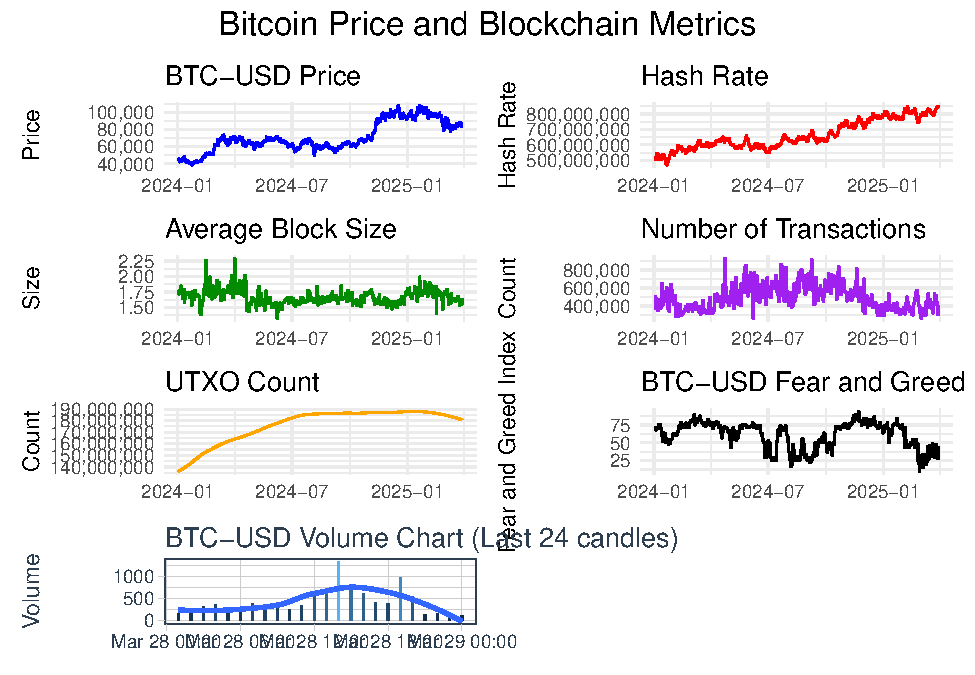
\includegraphics{REPORT_files/figure-latex/visual_analysis-1.pdf}

Find below the candletick chart of BTC-USD.

\begin{Shaded}
\begin{Highlighting}[]
\CommentTok{\# For more readability we are only plotting the last 24 candles}
\NormalTok{p7 }\OtherTok{\textless{}{-}}\NormalTok{ candles\_enhanced\_cleaned\_no\_na }\SpecialCharTok{\%\textgreater{}\%}
  \FunctionTok{tail}\NormalTok{(}\DecValTok{24}\NormalTok{) }\SpecialCharTok{\%\textgreater{}\%}
  \FunctionTok{mutate}\NormalTok{(}\AttributeTok{direction =} \FunctionTok{ifelse}\NormalTok{(close }\SpecialCharTok{\textgreater{}=}\NormalTok{ open, }\StringTok{"up"}\NormalTok{, }\StringTok{"down"}\NormalTok{)) }\SpecialCharTok{\%\textgreater{}\%}
  \FunctionTok{ggplot}\NormalTok{(}\FunctionTok{aes}\NormalTok{(}\AttributeTok{x =}\NormalTok{ time, }\AttributeTok{y =}\NormalTok{ close)) }\SpecialCharTok{+}
  \CommentTok{\# The shadows (wicks)}
  \FunctionTok{geom\_segment}\NormalTok{(}\FunctionTok{aes}\NormalTok{(}\AttributeTok{xend =}\NormalTok{ time, }\AttributeTok{y =}\NormalTok{ low, }\AttributeTok{yend =}\NormalTok{ high, }\AttributeTok{color =}\NormalTok{ direction), }\AttributeTok{size =} \FloatTok{0.5}\NormalTok{) }\SpecialCharTok{+}
  \CommentTok{\# The body}
  \FunctionTok{geom\_segment}\NormalTok{(}\FunctionTok{aes}\NormalTok{(}\AttributeTok{xend =}\NormalTok{ time, }\AttributeTok{y =}\NormalTok{ open, }\AttributeTok{yend =}\NormalTok{ close, }\AttributeTok{color =}\NormalTok{ direction), }\AttributeTok{size =} \DecValTok{5}\NormalTok{) }\SpecialCharTok{+}
  \FunctionTok{scale\_color\_manual}\NormalTok{(}\AttributeTok{values =} \FunctionTok{c}\NormalTok{(}\StringTok{"up"} \OtherTok{=} \StringTok{"darkgreen"}\NormalTok{, }\StringTok{"down"} \OtherTok{=} \StringTok{"red"}\NormalTok{)) }\SpecialCharTok{+}
  \FunctionTok{theme\_tq}\NormalTok{() }\SpecialCharTok{+}
  \FunctionTok{theme}\NormalTok{(}\AttributeTok{legend.position =} \StringTok{"none"}\NormalTok{) }\SpecialCharTok{+}
  \FunctionTok{labs}\NormalTok{(}
    \AttributeTok{title =} \StringTok{"BTC{-}USD Candlestick Chart (Last 24 Candles)"}\NormalTok{,}
    \AttributeTok{x =} \StringTok{"Time"}\NormalTok{,}
    \AttributeTok{y =} \StringTok{"Price"}
\NormalTok{  ) }\SpecialCharTok{+}
  \FunctionTok{scale\_y\_continuous}\NormalTok{(}\AttributeTok{labels =}\NormalTok{ scales}\SpecialCharTok{::}\NormalTok{comma)}
\end{Highlighting}
\end{Shaded}

And the plot of the different TA.

\begin{Shaded}
\begin{Highlighting}[]
\NormalTok{plot\_data\_ta }\OtherTok{\textless{}{-}}\NormalTok{ candles\_enhanced\_cleaned\_no\_na }\SpecialCharTok{\%\textgreater{}\%} \FunctionTok{tail}\NormalTok{(}\DecValTok{100}\NormalTok{)}

\CommentTok{\# ROC Plot}
\NormalTok{p\_roc }\OtherTok{\textless{}{-}}\NormalTok{ plot\_data\_ta }\SpecialCharTok{\%\textgreater{}\%}
  \FunctionTok{ggplot}\NormalTok{(}\FunctionTok{aes}\NormalTok{(}\AttributeTok{x =}\NormalTok{ time, }\AttributeTok{y =}\NormalTok{ roc)) }\SpecialCharTok{+}
  \FunctionTok{geom\_line}\NormalTok{() }\SpecialCharTok{+}
  \FunctionTok{labs}\NormalTok{(}\AttributeTok{title =} \StringTok{"Rate of Change (ROC)"}\NormalTok{, }\AttributeTok{y =} \StringTok{"ROC"}\NormalTok{) }\SpecialCharTok{+}
  \FunctionTok{theme\_tq}\NormalTok{() }\SpecialCharTok{+}
  \FunctionTok{theme}\NormalTok{(}\AttributeTok{axis.title.x =} \FunctionTok{element\_blank}\NormalTok{())}

\CommentTok{\# Bollinger Bands Plot}
\NormalTok{p\_bbands }\OtherTok{\textless{}{-}}\NormalTok{ plot\_data\_ta }\SpecialCharTok{\%\textgreater{}\%}
  \FunctionTok{ggplot}\NormalTok{(}\FunctionTok{aes}\NormalTok{(}\AttributeTok{x =}\NormalTok{ time, }\AttributeTok{y =}\NormalTok{ close)) }\SpecialCharTok{+}
  \FunctionTok{geom\_line}\NormalTok{(}\FunctionTok{aes}\NormalTok{(}\AttributeTok{y =}\NormalTok{ close), }\AttributeTok{color =} \StringTok{"blue"}\NormalTok{) }\SpecialCharTok{+} \CommentTok{\# Close price}
  \FunctionTok{geom\_ribbon}\NormalTok{(}\FunctionTok{aes}\NormalTok{(}\AttributeTok{ymin =}\NormalTok{ dn, }\AttributeTok{ymax =}\NormalTok{ up), }\AttributeTok{fill =} \StringTok{"grey"}\NormalTok{, }\AttributeTok{alpha =} \FloatTok{0.4}\NormalTok{) }\SpecialCharTok{+} \CommentTok{\# Bollinger Bands area}
  \FunctionTok{geom\_line}\NormalTok{(}\FunctionTok{aes}\NormalTok{(}\AttributeTok{y =}\NormalTok{ mavg), }\AttributeTok{color =} \StringTok{"red"}\NormalTok{, }\AttributeTok{linetype =} \StringTok{"dashed"}\NormalTok{) }\SpecialCharTok{+} \CommentTok{\# Moving Average}
  \FunctionTok{labs}\NormalTok{(}\AttributeTok{title =} \StringTok{"Bollinger Bands (BBands)"}\NormalTok{, }\AttributeTok{y =} \StringTok{"Price"}\NormalTok{) }\SpecialCharTok{+}
  \FunctionTok{theme\_tq}\NormalTok{() }\SpecialCharTok{+}
  \FunctionTok{theme}\NormalTok{(}\AttributeTok{axis.title.x =} \FunctionTok{element\_blank}\NormalTok{()) }\SpecialCharTok{+}
  \FunctionTok{scale\_y\_continuous}\NormalTok{(}\AttributeTok{labels =}\NormalTok{ scales}\SpecialCharTok{::}\NormalTok{comma)}

\CommentTok{\# MACD Plot}
\NormalTok{p\_macd }\OtherTok{\textless{}{-}}\NormalTok{ plot\_data\_ta }\SpecialCharTok{\%\textgreater{}\%}
  \FunctionTok{ggplot}\NormalTok{(}\FunctionTok{aes}\NormalTok{(}\AttributeTok{x =}\NormalTok{ time)) }\SpecialCharTok{+}
  \FunctionTok{geom\_line}\NormalTok{(}\FunctionTok{aes}\NormalTok{(}\AttributeTok{y =}\NormalTok{ macd), }\AttributeTok{color =} \StringTok{"blue"}\NormalTok{) }\SpecialCharTok{+}  \CommentTok{\# MACD line}
  \FunctionTok{geom\_line}\NormalTok{(}\FunctionTok{aes}\NormalTok{(}\AttributeTok{y =}\NormalTok{ signal), }\AttributeTok{color =} \StringTok{"red"}\NormalTok{, }\AttributeTok{linetype =} \StringTok{"dashed"}\NormalTok{) }\SpecialCharTok{+} \CommentTok{\# Signal line}
  \FunctionTok{geom\_col}\NormalTok{(}\FunctionTok{aes}\NormalTok{(}\AttributeTok{y =}\NormalTok{ macd }\SpecialCharTok{{-}}\NormalTok{ signal), }\AttributeTok{alpha =} \FloatTok{0.5}\NormalTok{) }\SpecialCharTok{+} \CommentTok{\# Histogram of MACD {-} Signal}
  \FunctionTok{labs}\NormalTok{(}\AttributeTok{title =} \StringTok{"MACD"}\NormalTok{, }\AttributeTok{y =} \StringTok{"Value"}\NormalTok{) }\SpecialCharTok{+}
  \FunctionTok{theme\_tq}\NormalTok{() }\SpecialCharTok{+}
  \FunctionTok{theme}\NormalTok{(}\AttributeTok{axis.title.x =} \FunctionTok{element\_blank}\NormalTok{())}

\CommentTok{\# RSI Plot}
\NormalTok{p\_rsi }\OtherTok{\textless{}{-}}\NormalTok{ plot\_data\_ta }\SpecialCharTok{\%\textgreater{}\%}
  \FunctionTok{ggplot}\NormalTok{(}\FunctionTok{aes}\NormalTok{(}\AttributeTok{x =}\NormalTok{ time, }\AttributeTok{y =}\NormalTok{ rsi)) }\SpecialCharTok{+}
  \FunctionTok{geom\_line}\NormalTok{() }\SpecialCharTok{+}
  \FunctionTok{geom\_hline}\NormalTok{(}\AttributeTok{yintercept =} \DecValTok{70}\NormalTok{, }\AttributeTok{linetype =} \StringTok{"dashed"}\NormalTok{, }\AttributeTok{color =} \StringTok{"red"}\NormalTok{) }\SpecialCharTok{+}  \CommentTok{\# Overbought level}
  \FunctionTok{geom\_hline}\NormalTok{(}\AttributeTok{yintercept =} \DecValTok{30}\NormalTok{, }\AttributeTok{linetype =} \StringTok{"dashed"}\NormalTok{, }\AttributeTok{color =} \StringTok{"darkgreen"}\NormalTok{) }\SpecialCharTok{+} \CommentTok{\# Oversold level}
  \FunctionTok{labs}\NormalTok{(}\AttributeTok{title =} \StringTok{"Relative Strength Index (RSI)"}\NormalTok{, }\AttributeTok{y =} \StringTok{"RSI"}\NormalTok{) }\SpecialCharTok{+}
  \FunctionTok{theme\_tq}\NormalTok{() }\SpecialCharTok{+}
  \FunctionTok{theme}\NormalTok{(}\AttributeTok{axis.title.x =} \FunctionTok{element\_blank}\NormalTok{())}

\CommentTok{\# Combine TA plots}
\NormalTok{combined\_ta\_plot }\OtherTok{\textless{}{-}}\NormalTok{ (p\_roc }\SpecialCharTok{/}\NormalTok{ p\_bbands) }\SpecialCharTok{|}\NormalTok{ (p\_macd }\SpecialCharTok{/}\NormalTok{ p\_rsi)}

\NormalTok{combined\_ta\_plot }\SpecialCharTok{+} \FunctionTok{plot\_annotation}\NormalTok{(}
  \AttributeTok{title =} \StringTok{"Technical Analysis Indicators (Last 100 Candles)"}\NormalTok{,}
  \AttributeTok{theme =} \FunctionTok{theme}\NormalTok{(}\AttributeTok{plot.title =} \FunctionTok{element\_text}\NormalTok{(}\AttributeTok{hjust =} \FloatTok{0.5}\NormalTok{, }\AttributeTok{size =} \DecValTok{16}\NormalTok{))}
\NormalTok{)}
\end{Highlighting}
\end{Shaded}

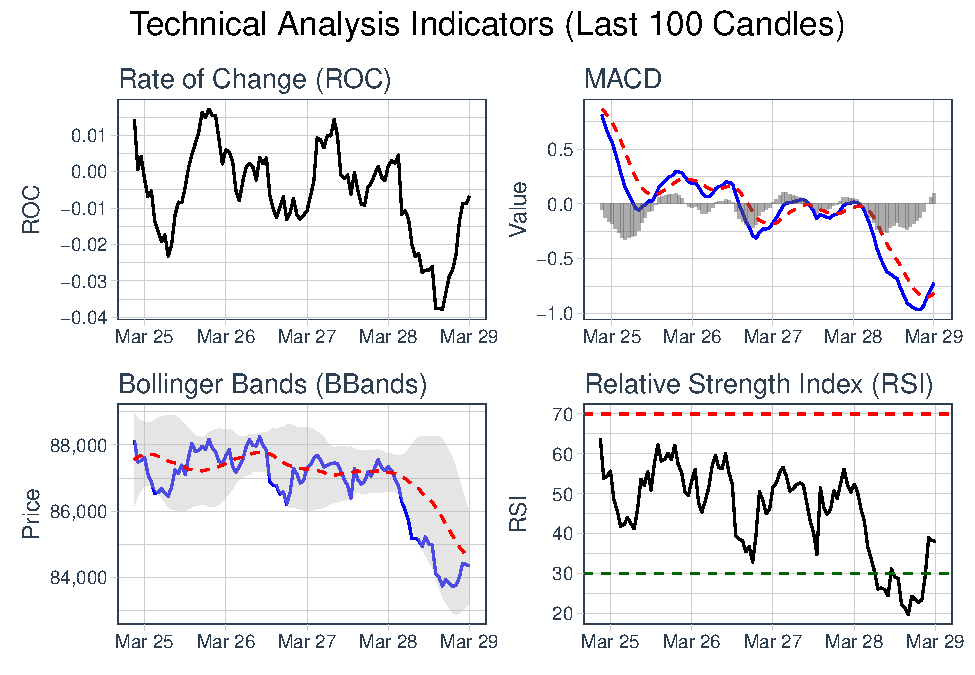
\includegraphics{REPORT_files/figure-latex/visual_ta-1.pdf} Comparing
with the data from TradingView it seems that all the charts are correct.

Let's now see how is the distribution of ``up'' and ``down'' candles.

\begin{Shaded}
\begin{Highlighting}[]
\NormalTok{candles\_enhanced\_cleaned\_no\_na }\SpecialCharTok{\%\textgreater{}\%}
    \FunctionTok{mutate}\NormalTok{(}\AttributeTok{direction =} \FunctionTok{ifelse}\NormalTok{(close }\SpecialCharTok{\textgreater{}=}\NormalTok{ open, }\StringTok{"up"}\NormalTok{, }\StringTok{"down"}\NormalTok{)) }\SpecialCharTok{\%\textgreater{}\%}
    \FunctionTok{summarise}\NormalTok{(}\AttributeTok{up =} \FunctionTok{sum}\NormalTok{(direction }\SpecialCharTok{==} \StringTok{"up"}\NormalTok{), }\AttributeTok{down =} \FunctionTok{sum}\NormalTok{(direction }\SpecialCharTok{==}
        \StringTok{"down"}\NormalTok{)) }\SpecialCharTok{\%\textgreater{}\%}
    \FunctionTok{pivot\_longer}\NormalTok{(}\AttributeTok{cols =} \FunctionTok{everything}\NormalTok{(), }\AttributeTok{names\_to =} \StringTok{"direction"}\NormalTok{,}
        \AttributeTok{values\_to =} \StringTok{"count"}\NormalTok{) }\SpecialCharTok{\%\textgreater{}\%}
    \FunctionTok{ggplot}\NormalTok{(}\FunctionTok{aes}\NormalTok{(}\AttributeTok{x =}\NormalTok{ direction, }\AttributeTok{y =}\NormalTok{ count, }\AttributeTok{fill =}\NormalTok{ direction)) }\SpecialCharTok{+}
    \FunctionTok{geom\_bar}\NormalTok{(}\AttributeTok{stat =} \StringTok{"identity"}\NormalTok{) }\SpecialCharTok{+} \FunctionTok{scale\_fill\_manual}\NormalTok{(}\AttributeTok{values =} \FunctionTok{c}\NormalTok{(}\AttributeTok{up =} \StringTok{"darkgreen"}\NormalTok{,}
    \AttributeTok{down =} \StringTok{"red"}\NormalTok{)) }\SpecialCharTok{+} \FunctionTok{theme\_minimal}\NormalTok{() }\SpecialCharTok{+} \FunctionTok{labs}\NormalTok{(}\AttributeTok{title =} \StringTok{"Number of Up vs Down Candles"}\NormalTok{,}
    \AttributeTok{x =} \StringTok{"Direction"}\NormalTok{, }\AttributeTok{y =} \StringTok{"Count"}\NormalTok{)}
\end{Highlighting}
\end{Shaded}

\includegraphics{REPORT_files/figure-latex/visual_repartion-1.pdf}

\begin{Shaded}
\begin{Highlighting}[]
\NormalTok{distribution\_data }\OtherTok{\textless{}{-}}\NormalTok{ candles\_enhanced\_cleaned\_no\_na }\SpecialCharTok{\%\textgreater{}\%}
    \FunctionTok{mutate}\NormalTok{(}\AttributeTok{direction =} \FunctionTok{ifelse}\NormalTok{(close }\SpecialCharTok{\textgreater{}=}\NormalTok{ open, }\StringTok{"up"}\NormalTok{, }\StringTok{"down"}\NormalTok{)) }\SpecialCharTok{\%\textgreater{}\%}
    \FunctionTok{summarise}\NormalTok{(}\AttributeTok{up =} \FunctionTok{sum}\NormalTok{(direction }\SpecialCharTok{==} \StringTok{"up"}\NormalTok{), }\AttributeTok{down =} \FunctionTok{sum}\NormalTok{(direction }\SpecialCharTok{==}
        \StringTok{"down"}\NormalTok{)) }\SpecialCharTok{\%\textgreater{}\%}
    \FunctionTok{mutate}\NormalTok{(}\AttributeTok{total =}\NormalTok{ up }\SpecialCharTok{+}\NormalTok{ down, }\AttributeTok{up\_percentage =}\NormalTok{ up}\SpecialCharTok{/}\NormalTok{total, }\AttributeTok{down\_percentage =}\NormalTok{ down}\SpecialCharTok{/}\NormalTok{total)}

\NormalTok{knitr}\SpecialCharTok{::}\FunctionTok{kable}\NormalTok{(distribution\_data, }\AttributeTok{format =} \StringTok{"simple"}\NormalTok{, }\AttributeTok{caption =} \StringTok{"Distribution of up and down candles"}\NormalTok{)}
\end{Highlighting}
\end{Shaded}

\begin{longtable}[]{@{}rrrrr@{}}
\caption{Distribution of up and down candles}\tabularnewline
\toprule\noalign{}
up & down & total & up\_percentage & down\_percentage \\
\midrule\noalign{}
\endfirsthead
\toprule\noalign{}
up & down & total & up\_percentage & down\_percentage \\
\midrule\noalign{}
\endhead
\bottomrule\noalign{}
\endlastfoot
5538 & 5302 & 10840 & 0.5108856 & 0.4891144 \\
\end{longtable}

We can notice that the distribution is not exacly 50\%.

\hypertarget{adding-lagged-candles}{%
\subsection{Adding lagged candles}\label{adding-lagged-candles}}

Our study aim at predicting the direction of a candle using the previous
candle's data and other features.

So we need to create a function to create a dataset containing lagged
candles. We also created another function to directly prepare the right
data.

\begin{Shaded}
\begin{Highlighting}[]
\NormalTok{add\_lagged\_candles }\OtherTok{\textless{}{-}} \ControlFlowTok{function}\NormalTok{(enhanced\_clean\_dataset, n\_lag) \{}
\NormalTok{    dataset\_with\_lagged\_candles }\OtherTok{\textless{}{-}}\NormalTok{ enhanced\_clean\_dataset}

    \ControlFlowTok{for}\NormalTok{ (i }\ControlFlowTok{in} \DecValTok{1}\SpecialCharTok{:}\NormalTok{n\_lag) \{}
\NormalTok{        dataset\_with\_lagged\_candles[[}\FunctionTok{paste0}\NormalTok{(}\StringTok{"body\_size\_lag\_"}\NormalTok{,}
\NormalTok{            i)]] }\OtherTok{\textless{}{-}} \FunctionTok{lag}\NormalTok{(dataset\_with\_lagged\_candles}\SpecialCharTok{$}\NormalTok{body\_size,}
\NormalTok{            i)}
\NormalTok{        dataset\_with\_lagged\_candles[[}\FunctionTok{paste0}\NormalTok{(}\StringTok{"upper\_shadow\_size\_lag\_"}\NormalTok{,}
\NormalTok{            i)]] }\OtherTok{\textless{}{-}} \FunctionTok{lag}\NormalTok{(dataset\_with\_lagged\_candles}\SpecialCharTok{$}\NormalTok{upper\_shadow\_size,}
\NormalTok{            i)}
\NormalTok{        dataset\_with\_lagged\_candles[[}\FunctionTok{paste0}\NormalTok{(}\StringTok{"lower\_shadow\_size\_lag\_"}\NormalTok{,}
\NormalTok{            i)]] }\OtherTok{\textless{}{-}} \FunctionTok{lag}\NormalTok{(dataset\_with\_lagged\_candles}\SpecialCharTok{$}\NormalTok{lower\_shadow\_size,}
\NormalTok{            i)}
\NormalTok{        dataset\_with\_lagged\_candles[[}\FunctionTok{paste0}\NormalTok{(}\StringTok{"direction\_lag\_"}\NormalTok{,}
\NormalTok{            i)]] }\OtherTok{\textless{}{-}} \FunctionTok{lag}\NormalTok{(dataset\_with\_lagged\_candles}\SpecialCharTok{$}\NormalTok{direction,}
\NormalTok{            i)}
\NormalTok{        dataset\_with\_lagged\_candles[[}\FunctionTok{paste0}\NormalTok{(}\StringTok{"volume\_lag\_"}\NormalTok{, i)]] }\OtherTok{\textless{}{-}} \FunctionTok{lag}\NormalTok{(dataset\_with\_lagged\_candles}\SpecialCharTok{$}\NormalTok{volume,}
\NormalTok{            i)}
\NormalTok{        dataset\_with\_lagged\_candles[[}\FunctionTok{paste0}\NormalTok{(}\StringTok{"value\_lag\_"}\NormalTok{, i)]] }\OtherTok{\textless{}{-}} \FunctionTok{lag}\NormalTok{(dataset\_with\_lagged\_candles}\SpecialCharTok{$}\NormalTok{value,}
\NormalTok{            i)}
\NormalTok{        dataset\_with\_lagged\_candles[[}\FunctionTok{paste0}\NormalTok{(}\StringTok{"close\_lag\_"}\NormalTok{, i)]] }\OtherTok{\textless{}{-}} \FunctionTok{lag}\NormalTok{(dataset\_with\_lagged\_candles}\SpecialCharTok{$}\NormalTok{close,}
\NormalTok{            i)}
\NormalTok{        dataset\_with\_lagged\_candles[[}\FunctionTok{paste0}\NormalTok{(}\StringTok{"hash\_rate\_lag\_"}\NormalTok{,}
\NormalTok{            i)]] }\OtherTok{\textless{}{-}} \FunctionTok{lag}\NormalTok{(dataset\_with\_lagged\_candles}\SpecialCharTok{$}\NormalTok{hash\_rate,}
\NormalTok{            i)}
\NormalTok{        dataset\_with\_lagged\_candles[[}\FunctionTok{paste0}\NormalTok{(}\StringTok{"avg\_block\_size\_lag\_"}\NormalTok{,}
\NormalTok{            i)]] }\OtherTok{\textless{}{-}} \FunctionTok{lag}\NormalTok{(dataset\_with\_lagged\_candles}\SpecialCharTok{$}\NormalTok{avg\_block\_size,}
\NormalTok{            i)}
\NormalTok{        dataset\_with\_lagged\_candles[[}\FunctionTok{paste0}\NormalTok{(}\StringTok{"n\_transactions\_lag\_"}\NormalTok{,}
\NormalTok{            i)]] }\OtherTok{\textless{}{-}} \FunctionTok{lag}\NormalTok{(dataset\_with\_lagged\_candles}\SpecialCharTok{$}\NormalTok{n\_transactions,}
\NormalTok{            i)}
\NormalTok{        dataset\_with\_lagged\_candles[[}\FunctionTok{paste0}\NormalTok{(}\StringTok{"utxo\_count\_lag\_"}\NormalTok{,}
\NormalTok{            i)]] }\OtherTok{\textless{}{-}} \FunctionTok{lag}\NormalTok{(dataset\_with\_lagged\_candles}\SpecialCharTok{$}\NormalTok{utxo\_count,}
\NormalTok{            i)}
\NormalTok{        dataset\_with\_lagged\_candles[[}\FunctionTok{paste0}\NormalTok{(}\StringTok{"open\_lag\_"}\NormalTok{, i)]] }\OtherTok{\textless{}{-}} \FunctionTok{lag}\NormalTok{(dataset\_with\_lagged\_candles}\SpecialCharTok{$}\NormalTok{open,}
\NormalTok{            i)}
\NormalTok{        dataset\_with\_lagged\_candles[[}\FunctionTok{paste0}\NormalTok{(}\StringTok{"high\_lag\_"}\NormalTok{, i)]] }\OtherTok{\textless{}{-}} \FunctionTok{lag}\NormalTok{(dataset\_with\_lagged\_candles}\SpecialCharTok{$}\NormalTok{high,}
\NormalTok{            i)}
\NormalTok{        dataset\_with\_lagged\_candles[[}\FunctionTok{paste0}\NormalTok{(}\StringTok{"low\_lag\_"}\NormalTok{, i)]] }\OtherTok{\textless{}{-}} \FunctionTok{lag}\NormalTok{(dataset\_with\_lagged\_candles}\SpecialCharTok{$}\NormalTok{low,}
\NormalTok{            i)}
\NormalTok{        dataset\_with\_lagged\_candles[[}\FunctionTok{paste0}\NormalTok{(}\StringTok{"roc\_lag\_"}\NormalTok{, i)]] }\OtherTok{\textless{}{-}} \FunctionTok{lag}\NormalTok{(dataset\_with\_lagged\_candles}\SpecialCharTok{$}\NormalTok{roc,}
\NormalTok{            i)}
\NormalTok{        dataset\_with\_lagged\_candles[[}\FunctionTok{paste0}\NormalTok{(}\StringTok{"macd\_lag\_"}\NormalTok{, i)]] }\OtherTok{\textless{}{-}} \FunctionTok{lag}\NormalTok{(dataset\_with\_lagged\_candles}\SpecialCharTok{$}\NormalTok{macd,}
\NormalTok{            i)}
\NormalTok{        dataset\_with\_lagged\_candles[[}\FunctionTok{paste0}\NormalTok{(}\StringTok{"signal\_lag\_"}\NormalTok{, i)]] }\OtherTok{\textless{}{-}} \FunctionTok{lag}\NormalTok{(dataset\_with\_lagged\_candles}\SpecialCharTok{$}\NormalTok{signal,}
\NormalTok{            i)}
\NormalTok{        dataset\_with\_lagged\_candles[[}\FunctionTok{paste0}\NormalTok{(}\StringTok{"rsi\_lag\_"}\NormalTok{, i)]] }\OtherTok{\textless{}{-}} \FunctionTok{lag}\NormalTok{(dataset\_with\_lagged\_candles}\SpecialCharTok{$}\NormalTok{rsi,}
\NormalTok{            i)}
\NormalTok{        dataset\_with\_lagged\_candles[[}\FunctionTok{paste0}\NormalTok{(}\StringTok{"up\_bband\_lag\_"}\NormalTok{,}
\NormalTok{            i)]] }\OtherTok{\textless{}{-}} \FunctionTok{lag}\NormalTok{(dataset\_with\_lagged\_candles}\SpecialCharTok{$}\NormalTok{up, i)}
\NormalTok{        dataset\_with\_lagged\_candles[[}\FunctionTok{paste0}\NormalTok{(}\StringTok{"mavg\_lag\_"}\NormalTok{, i)]] }\OtherTok{\textless{}{-}} \FunctionTok{lag}\NormalTok{(dataset\_with\_lagged\_candles}\SpecialCharTok{$}\NormalTok{mavg,}
\NormalTok{            i)}
\NormalTok{        dataset\_with\_lagged\_candles[[}\FunctionTok{paste0}\NormalTok{(}\StringTok{"dn\_bband\_lag\_"}\NormalTok{,}
\NormalTok{            i)]] }\OtherTok{\textless{}{-}} \FunctionTok{lag}\NormalTok{(dataset\_with\_lagged\_candles}\SpecialCharTok{$}\NormalTok{dn, i)}
\NormalTok{        dataset\_with\_lagged\_candles[[}\FunctionTok{paste0}\NormalTok{(}\StringTok{"pctB\_lag\_"}\NormalTok{, i)]] }\OtherTok{\textless{}{-}} \FunctionTok{lag}\NormalTok{(dataset\_with\_lagged\_candles}\SpecialCharTok{$}\NormalTok{pctB,}
\NormalTok{            i)}
\NormalTok{    \}}

\NormalTok{    dataset\_with\_lagged\_candles}
\NormalTok{\}}

\NormalTok{prepare\_dataset }\OtherTok{\textless{}{-}} \ControlFlowTok{function}\NormalTok{(candles\_data, fear\_and\_greed\_index\_data,}
\NormalTok{    hash\_rate\_data, average\_block\_size\_data, n\_transactions\_data,}
\NormalTok{    utxo\_count\_data) \{}
\NormalTok{    enhanced\_clean\_dataset }\OtherTok{\textless{}{-}} \FunctionTok{enhance\_dataset}\NormalTok{(candles\_data, fear\_and\_greed\_index\_data,}
\NormalTok{        hash\_rate\_data, average\_block\_size\_data, n\_transactions\_data,}
\NormalTok{        utxo\_count\_data)}
\NormalTok{    enhanced\_clean\_dataset\_without\_na }\OtherTok{\textless{}{-}}\NormalTok{ enhanced\_clean\_dataset }\SpecialCharTok{\%\textgreater{}\%}
        \FunctionTok{drop\_na}\NormalTok{()}
\NormalTok{    dataset\_with\_lagged\_candles }\OtherTok{\textless{}{-}} \FunctionTok{add\_lagged\_candles}\NormalTok{(enhanced\_clean\_dataset\_without\_na,}
        \DecValTok{15}\NormalTok{)}
\NormalTok{    dataset\_with\_lagged\_candles\_without\_na }\OtherTok{\textless{}{-}}\NormalTok{ dataset\_with\_lagged\_candles }\SpecialCharTok{\%\textgreater{}\%}
        \FunctionTok{drop\_na}\NormalTok{()}
\NormalTok{    dataset\_with\_lagged\_candles\_without\_na}
\NormalTok{\}}
\end{Highlighting}
\end{Shaded}

Using the function \texttt{prepare\_dataset} and the we can have
directly the final dataset with lagged data.

\hypertarget{test-and-training-datasets}{%
\subsection{Test and training
datasets}\label{test-and-training-datasets}}

We put together the code to fix the fear\_and\_greed\_index and to
prepare the datasets and split them in train and test sets.

\begin{Shaded}
\begin{Highlighting}[]
\NormalTok{fear\_and\_greed\_index\_date\_before\_na }\OtherTok{\textless{}{-}}\NormalTok{ fear\_and\_greed\_index }\SpecialCharTok{\%\textgreater{}\%}
    \FunctionTok{filter}\NormalTok{(timestamp }\SpecialCharTok{==} \FunctionTok{as.Date}\NormalTok{(}\StringTok{"2024{-}10{-}25"}\NormalTok{))}
\NormalTok{fear\_and\_greed\_index\_date\_after\_na }\OtherTok{\textless{}{-}}\NormalTok{ fear\_and\_greed\_index }\SpecialCharTok{\%\textgreater{}\%}
    \FunctionTok{filter}\NormalTok{(timestamp }\SpecialCharTok{==} \FunctionTok{as.Date}\NormalTok{(}\StringTok{"2024{-}10{-}27"}\NormalTok{))}
\NormalTok{fear\_and\_greed\_value\_date\_na }\OtherTok{\textless{}{-}} \FunctionTok{mean}\NormalTok{(}\FunctionTok{c}\NormalTok{(fear\_and\_greed\_index\_date\_before\_na}\SpecialCharTok{$}\NormalTok{value,}
\NormalTok{    fear\_and\_greed\_index\_date\_after\_na}\SpecialCharTok{$}\NormalTok{value))}

\NormalTok{fear\_and\_greed\_index\_corrected }\OtherTok{\textless{}{-}}\NormalTok{ fear\_and\_greed\_index }\SpecialCharTok{\%\textgreater{}\%}
    \FunctionTok{bind\_rows}\NormalTok{(}\FunctionTok{tibble}\NormalTok{(}\AttributeTok{timestamp =}\NormalTok{ date\_na, }\AttributeTok{value =}\NormalTok{ fear\_and\_greed\_value\_date\_na,}
        \AttributeTok{value\_classification =} \StringTok{"Greed"}\NormalTok{))}

\NormalTok{project\_dataset }\OtherTok{\textless{}{-}} \FunctionTok{prepare\_dataset}\NormalTok{(candles, fear\_and\_greed\_index\_corrected,}
\NormalTok{    hash\_rate, average\_block\_size, n\_transactions, utxo\_count)}
\end{Highlighting}
\end{Shaded}

\begin{verbatim}
## Warning in coerce_to_tibble(ret, date_col_name, time_zone, col_rename): Could not rename columns. The function name will be used. 
##   Is the length of `col_rename` the same as the number of columns returned from the `mutate_fun`?
\end{verbatim}

\begin{Shaded}
\begin{Highlighting}[]
\FunctionTok{sum}\NormalTok{(}\FunctionTok{is.na}\NormalTok{(project\_dataset))}
\end{Highlighting}
\end{Shaded}

\begin{verbatim}
## [1] 0
\end{verbatim}

\begin{Shaded}
\begin{Highlighting}[]
\FunctionTok{nrow}\NormalTok{(project\_dataset)}
\end{Highlighting}
\end{Shaded}

\begin{verbatim}
## [1] 10825
\end{verbatim}

\begin{Shaded}
\begin{Highlighting}[]
\FunctionTok{nrow}\NormalTok{(candles)}
\end{Highlighting}
\end{Shaded}

\begin{verbatim}
## [1] 10873
\end{verbatim}

\begin{Shaded}
\begin{Highlighting}[]
\NormalTok{test\_index }\OtherTok{\textless{}{-}} \FunctionTok{createDataPartition}\NormalTok{(}\AttributeTok{y =}\NormalTok{ project\_dataset}\SpecialCharTok{$}\NormalTok{direction,}
    \AttributeTok{times =} \DecValTok{1}\NormalTok{, }\AttributeTok{p =} \FloatTok{0.2}\NormalTok{, }\AttributeTok{list =} \ConstantTok{FALSE}\NormalTok{)}
\NormalTok{train\_set }\OtherTok{\textless{}{-}}\NormalTok{ project\_dataset[}\SpecialCharTok{{-}}\NormalTok{test\_index, ]}
\NormalTok{test\_set }\OtherTok{\textless{}{-}}\NormalTok{ project\_dataset[test\_index, ]}
\end{Highlighting}
\end{Shaded}

The number of rows reduced since adding lags introduced a lot of NAs in
the first rows, NAs that we removed. Also we decided not to use cross
validation to reduce the time of training for the different machine
learnings algorithms. Note that we initiated already the project using
\texttt{set.seed(1)} part of the global variables.

\hypertarget{machine-learning-algorithms}{%
\subsection{Machine learning
algorithms}\label{machine-learning-algorithms}}

Based on some shallow research on the press, we selected the following
machine learnings algorithms that seems to work better with our type of
dataset:

\begin{itemize}
\item
  Generalized Linear Model (GLM)
\item
  Decision Tree (DT)
\item
  Random Forest (RF)
\item
  K-nearest neighbor (KNN)
\item
  Gradient boosting (GBM)
\end{itemize}

TODO add links reference
\url{https://www.neuroquantology.com/open-access/An+Optimized+Machine+Learning+Model+for+Candlestick+Chart+Analysis+to+Predict+Stock+Market+Trends_9861/?download=true}
\url{https://arxiv.org/pdf/1606.00930}

We will also compare these algorithms with Random guess as a reference.

\hypertarget{utility-functions}{%
\subsection{Utility functions}\label{utility-functions}}

Since we want to compare each algorithms for a different set of features
we need a function to create the formula that we will pass to the
machine learning function.

\end{document}
